\documentclass[a4paper,11pt]{article}
\usepackage[T1]{fontenc}
\usepackage[utf8]{inputenc}
\usepackage{lmodern}
\usepackage{hyperref}
\usepackage{graphicx}
\usepackage{rotating}
\usepackage{listings}
\usepackage{color}
\usepackage{appendix}
\usepackage{caption}
\usepackage{float}
\usepackage{listings}

% Swedish
\usepackage[swedish]{babel}

% Table of contents depth 3 levels: A.B.C
\setcounter{tocdepth}{3}

\lstset{ %
language=VHDL,                  % the language of the code
basicstyle=\tiny,       	% the size of the fonts that are used for the code
numbers=left,                   % where to put the line-numbers
numberstyle=\tiny,      	% the size of the fonts that are used for the line-numbers
stepnumber=5,                   % the step between two line-numbers. If it's 1, each line will be numbered
numbersep=5pt,                  % how far the line-numbers are from the code
backgroundcolor=\color{white},  % choose the background color. You must add \usepackage{color}
showspaces=false,               % show spaces adding particular underscores
showstringspaces=false,         % underline spaces within strings
showtabs=false,                 % show tabs within strings adding particular underscores
frame=single,                   % adds a frame around the code
tabsize=2,                      % sets default tabsize to 2 spaces
captionpos=t,                   % sets the caption-position to top
breaklines=true,                % sets automatic line breaking
breakatwhitespace=false,        % sets if automatic breaks should only happen at whitespace
title=\lstname,                 % show the filename of files included with \lstinputlisting; also try caption instead of title
}


\begin{document}

\title{{\huge Sommarstugekoll} \\
	Digital Konstruktion EDA234 \\ Grupp 2}
\author{Fredrik Brosser, Karl Buchka, Andreas Henriksson, Johan Wolgers \\ \\
   	Chalmers Tekniska Högskola \\ \\
	\begin{tabular}{l c r}
		\texttt{frebro} & \texttt{@} & \texttt{student.chalmers.se}\\
		\texttt{karlbu} & \texttt{@} & \texttt{student.chalmers.se}\\
		\texttt{henriksa} & \texttt{@} & \texttt{student.chalmers.se}\\
		\texttt{wolgers} & \texttt{@} & \texttt{student.chalmers.se}\\\\
	\end{tabular}
	}
	
 \thispagestyle{empty}
\pagebreak

\maketitle
 \thispagestyle{empty}
\pagebreak

\begin{center}
	{\noindent \bf Sammanfattning}
\end{center}

	Ett system för temperaturavläsning och relästyrning beskrivs genom denna rapport. Systemet är åtkomligt och styrbart via telefon genom DTMF (Dual Tone Multiple Frequency). Systemets funktion består i att informera användaren om aktuella temperaturer från två temperatursensorer samt ge användaren möjlighet att via telefon styra utgångarna (till/från) för exempelvis värmeelement eller belysning. Styrning och återkoppling utbytes genom en telefonlinje, POTS (Plain Old Telephone Service) med hjälp av DTMF.

En tänkt tillämpning för produkten:
\begin{list}{*}{}
\item Systemet inkopplas innan avfärd från sommarstugan och befinner sig i viloläge. 
\item Användaren kan då denne önskar ringa upp systemet som på anmodan returnerar temperatur från någon av temperaturgivarna.
\item Användaren kan sedan genom sin knapptelefon aktivera eller avaktivera någon av utgångarna för att på så sätt slå till värme, belysning eller vad som anslutits till funktionsutgångarna.
\end{list}

\begin{center}
	{\noindent \bf Abstract}
\end{center}

	The system described in this report is an automated domestic temperature monitoring system, accessible and controllable via
	telephone. The main function of the system is to inform the user of the current temperatures
	at the points of measurement, and also to give the user remote binary control (on/off) of a number of external
	functions. These functions could for example be heating systems, radiators, or lighting. Information- and control data
	is exchanged via a standard analog telephone connection, POTS (Plain Old Telephone Service) using DTMF (Dual Tone, Multiple Frequency).

	A specific, practical application is of the concerned holiday home owner wanting to monitor and control the temperature 
	in his or her vacation property. Using Sommarstugekoll it is possible to keep heating expenditures to a minimum while at 
	the same time reducing the risk of temperature related property damage such as burst water pipes.

	Should the owner wish to visit the property, he or she needs only to dial the house telephone prior to arrival and instruct the system to raise
	the interior temperature to a comfortable level. 

\pagebreak

 \thispagestyle{empty}
	\tableofcontents
 \thispagestyle{empty}

\pagebreak

\setcounter{page}{1}
\section{Introduktion}

	Konstruktionsprojektet utförs inom kursen ``Digital Konstruktion, EDA234'' vid Chalmers Tekniska Högskola. Uppgiften består att inom gruppen om 4 personer konstruera och dokumentera
	ett digitalt system utifrån en specifikation, med fokus på huvudfunktionalitet i det digitala området. För en beskrivning av arbetsfördelningen inom gruppen, se Appendix~\ref{sec:arbetsSec}. Utvecklingen sker på ett färdigt utvecklingskort vilket sedan kompletteras med externa kretsar och programmeras för att nå kravspecefikationen. Logikkretsen som används är en Xilinx XC9572XL CPLD, och utveckligen sker i huvudsak med VHDL i Xilinx ISE-miljön samt i ModelSim för simuleringar. Rapporten är uppdelad i abstraktionslager med fördjupningar i de senare avsnitten. 

	En handhavandeinstruktion återfinns bifogad i Appendix~\ref{sec:Manual}.

\pagebreak

\section{Kravspecifikation och systembeskrivning}
	Systemet består av en styrenhet placerad på två CPLD med anslutning till telefonnätet. Styrenheten har med hjälp av en DTMF avkodare möjlighet att tolka användarens telefonknapptryckningar på distans. Vidare kan användaren genom dessa knapptryckningar skicka signal för att hämta värde från någon av de två temperaturgivarna anslutna med entrådsbus. En röstenhet läser sedan upp ett förinspelat meddelande för respektive temperatur. Vidare kan användaren också starta eller stoppa någon av de funktionsutgångar som finns till hands, användaren får då akustisk återkoppling om aktuell status för funktionsutgången via samma ljudmodul.

Funktionsutgångarna kan också styras lokalt med bifogade knappsatsen. Aktuell status för funktionsutgångarna visas med lysdioder. 

	\subsection{Tolkning och definition av kravspecifikation}

		Inom det tilltänkta användningsområdet, ett fritidshus med POTS-linje som under större delen av året endast nyttjas tillfälligtvis, är det rimligt med en minsta temperatur om $5-10\,^{\circ}\mathrm{C}$ då ingen vistas i huset. Vidare bör det vara önskvärt att ha möjlighet att slå till normal värme innan ett besök, kunna kontrollera att det blivit varmt samt att kontrollera att temperaturen är över $0\,^{\circ}\mathrm{C}$. Systemet kan därför tolka en temperatur om $\pm 32\,^{\circ}\mathrm{C}$ från givarna med en upplösning om $\pm 1\,^{\circ}\mathrm{C}$. Senast avlästa temperatur visas också binärt på LED-displayen. Systemet matas med en spänning om $5\,V$ DC, då systemet är till indikeras detta med en lysdiod.

	\subsection{Uppdelning}

	Systemet är uppdelat i ett antal delblock (moduler) och är konstruerat för att vara så modulärt som möjligt.
	I tabell ~\ref{tab:uppdelningstabell} nedan finns en beskrivning över hur de olika modulerna är uppdelade på de två CPLD:erna. Varje modul är mer
	utförligt beskriven under sektion~\ref{sec:Funktionsenheter} \nameref{sec:Funktionsenheter}. 

	I blockschema som återfinns i figur~\ref{fig:blocks1} och~\ref{fig:blocks2} visas respektive modul och uppdelningen på två CPLD samt dess kommunikationsvägar. För större figurer, se Appendix~\ref{sec:BlockAppendix}.\\

	\begin{figure} [H]
		  	
			\centering
			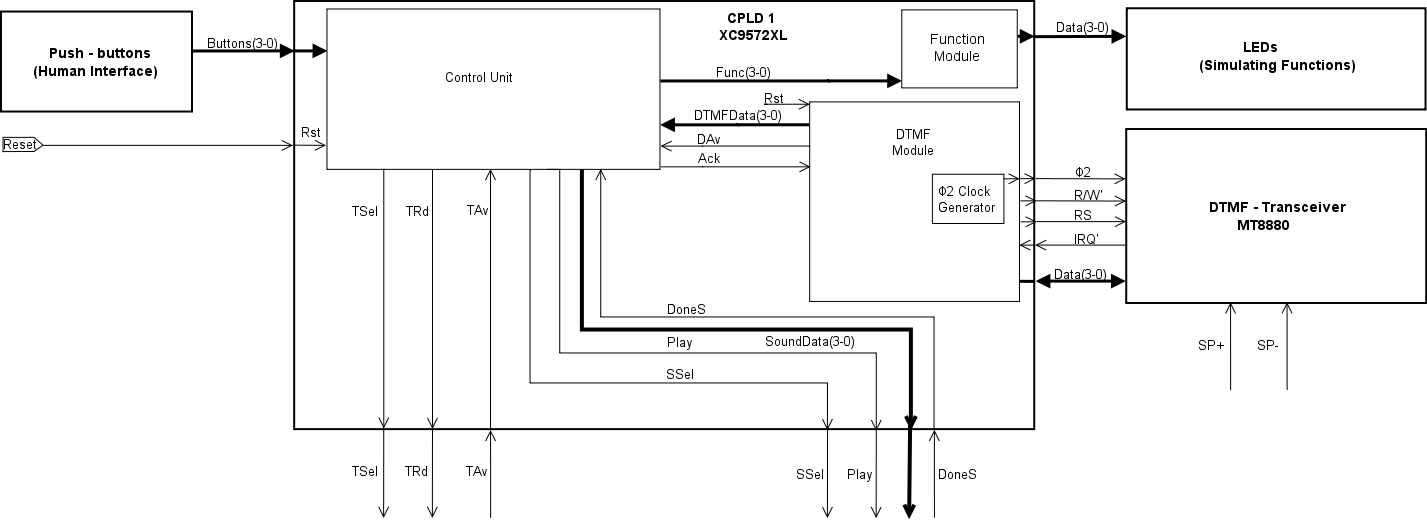
\includegraphics[width=1\textwidth, height = 0.40\textwidth]{BlockDiagramCPLD1.png}
		  	\caption{Blockdiagram för CPLD1}
			\label{fig:blocks1}
	\end{figure}

	\begin{figure}[H]
		  	
			\centering
			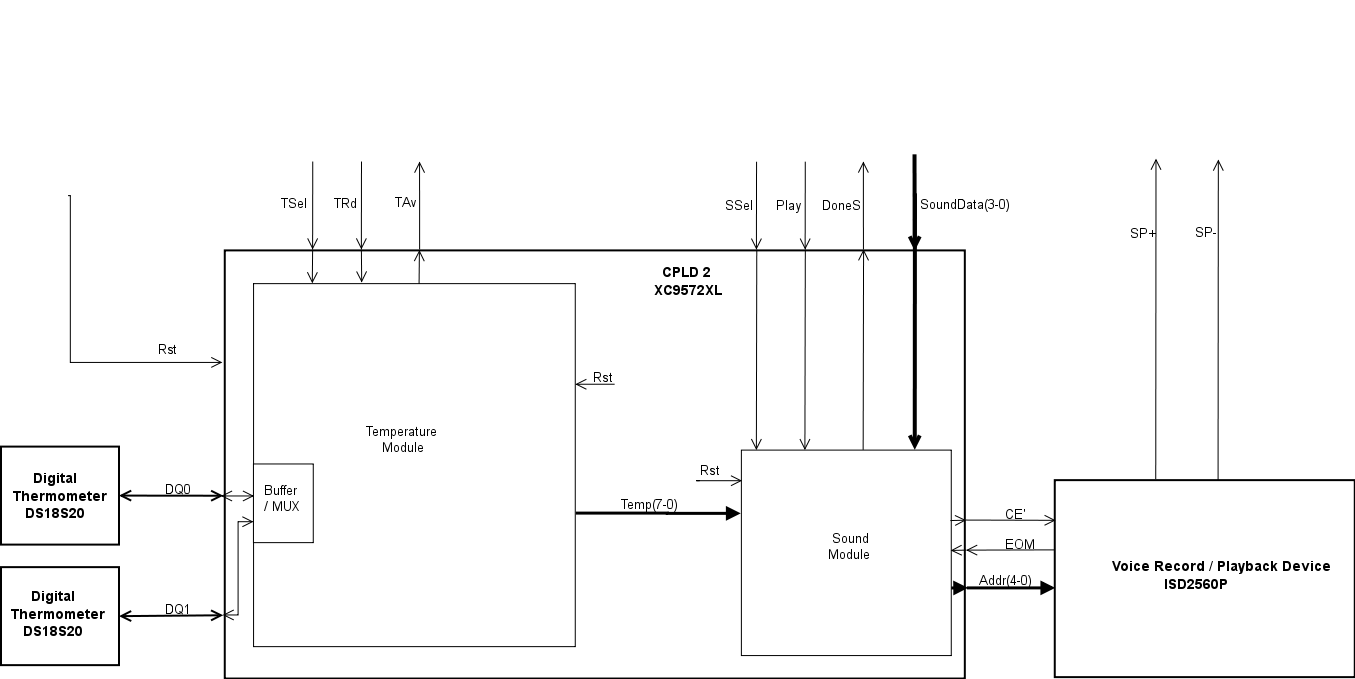
\includegraphics[width=1\textwidth, height = 0.40\textwidth]{BlockDiagramCPLD2.png}
			\caption{Blockdiagram för CPLD2}
			\label{fig:blocks2}
	\end{figure}

	\begin{table} [H]
		
		\caption{Respektive CPLDs moduler och uppgifter} 
		\label{tab:uppdelningstabell}
	\begin{tabular}{l l}
		
		{\bf CPLD1} \\
		Modul	& Funktion	\\
		\hline
		Styrenhet	& Samordnar systemets funktion \\
		DTMF-modul & Tar emot DTMF-signaler via POTS \\
		Funktionsmodul	& Hanterar funktionsutgångarna \\
		Knappmodul	& Hanterar tryckningar på knappsatsen \\
		\\
		{\bf CPLD2} \\
		Modul	& Funktion	\\
		\hline
		Temperaturmodul	& Initierar, läser och presenterar temperatur \\
		Ljudmodul	& Hanterar styrning av extern ljudkrets \\
		
	\end{tabular}
	\end{table}
	
	Systemet är uppdelat enligt ``dataväg-styrenhet-modellen'', där designprincipen går ut på att skilja styrsignaler
	och dataflödeskontroll (styrenheten) från datan som forslas genom systemet (datavägen). Systemet skickar temperaturdata från temperaturmodulen till ljudmodulen samt adressdata till ljudlagringsenheten från ljudmodulen. Detta flöde kontrolleras från styrenheten via
	enkla styrsignaler. Viss data, i form av indata från användargränssnitt och styrsignaler till funktionsutgångar, passerar dock genom styrenheten.

	\subsection{Arbetsflöde}

I sitt viloläge väntar systemet på inkommande samtal. Då samtal mottages börjar systemet med att läsa upp ett antal ljudklipp med aktuella temperaturer, och erbjuder sedan användaren möjligheten till att styra de externa funktionerna. Telefonen skickar ut DTMF-signaler, som läses och avkodas av DTMF-transceivern, MT8880C, vilken avkodar tvåtonssignalerna för att identifiera nedtryckt knapp och sända ut denna på databussen till DTMF-modulen. 

Då användaren trycker ned en knapp kontrollerar styrenheten om knapptryckningen motsvarar ett funktionskommando (funktion till eller från), i så fall sätts statusen för respektive funktionsutgång, annars återgår systemet till att invänta nytt kommando.

\pagebreak

\section{Funktionsenheter}
\label{sec:Funktionsenheter}

Systemet är som tidigare nämnt uppdelat i sex funktionsenheter: funktionsmodul, knappsatsmodul, styrenhet, DTMF-modul, ljudmodul och temperaturmodul.
Dessa presenteras närmare i respektive avsnitt nedan.

	\subsection{Dataväg}
	Temperaturdatan avläses från temperatursensorerna och skickas till temperaturmodulen. Denna skickar sedan datan till ljudmodulen, för vidare uppläsning via ljudlagringskretsen, ISD2560P. Denna data skickas aldrig genom, men kontrolleras av, styrenheten. Den rena datavägen i systemet är alltså här begränsad till CPLD2.
	
	\subsection{Styrenhet}

	Styrenheten kontrollerar och ger styrsignaler för att hantera de övriga systemdelarna. Syftet är att ge en lätt överblick över hela körcykeln, där styrenheten har kontroll över funktionerna via en rad styr-, available- och acknowledgesignaler. Styrenheten får även indata från knappsats och DTMF-mottagare via respektive modul som presenterar data för styrenheten. Denna indata är skild från datavägen (temperaturinformation), och meddelar styrenheten om nästföljande steg, dvs. reagera i enlighet med användarsignaler. Se figur~\ref{fig:CUFlowChart} för flödesschema.

		\begin{figure}[H]
		  \centering
		      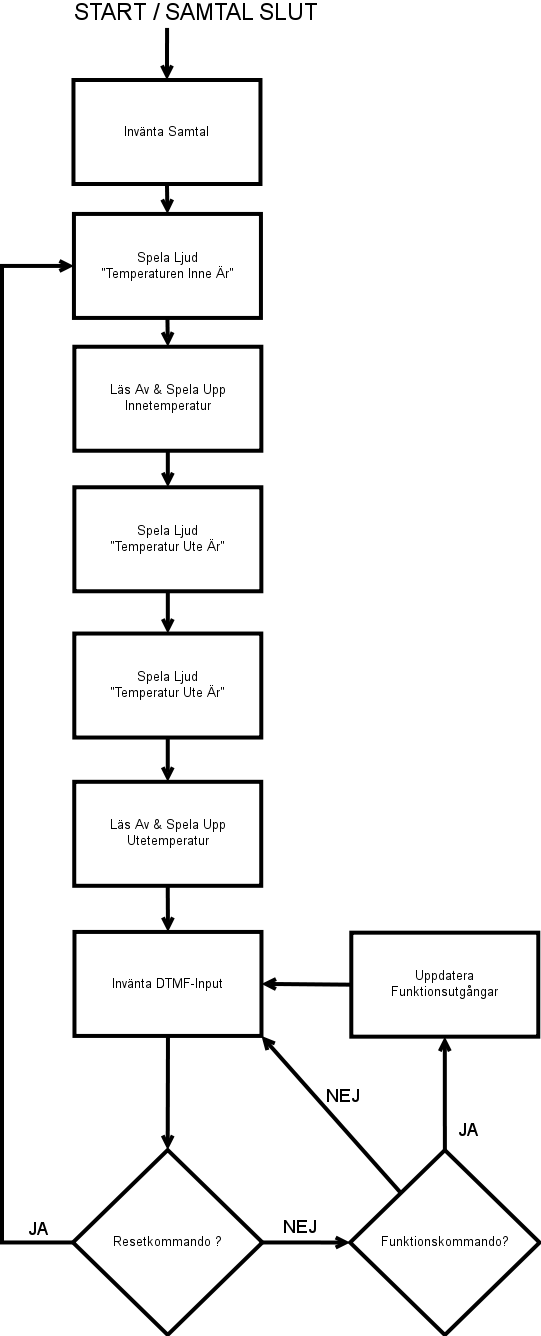
\includegraphics[scale=0.35, angle=0]{ControlUnitFlowChart.png}
		  	\caption{Högnivå-flödesdiagram för styrenhet}
			\label{fig:CUFlowChart}
		\end{figure}

	\subsubsection{Uppbyggnad}

	Styrenheten är i sin tur modulärt uppbyggd, och har ett väl avgränsat interface mot varje annan delmodul, men fungerar samtidigt som en samordnare mellan de olika modulerna. För en ingående grafisk beskrivning av den bakomliggande tillståndsmaskinen, se sektion~\ref{sec:Tillstandsmaskiner} ~\nameref{sec:Tillstandsmaskiner}.

	\subsection{DTMF-modul}
		
	DTMF-modulen i CPLD1 är ansvarig för att hantera kommunikation med telefonen och därmed också med användaren.
	När användaren trycker ner en knapp på telefonen genereras en DTMF-signal som uppfattas och avkodas av DTMF-modulen vilken sedan presenterar den mottagna indatan för styrenheten.
		
	\subsubsection{Initiering}

	DTMF-modulen måste genomgå en initieringssekvens minst 100 ms efter spänningspåslag. Detta sker med hjälp av
	en extern tryckknapp, som beskrivet i användarmanualen. Under hela initieringen är Chip Select satt låg
	och RS0 satt hög. Initieringscykeln börjar med att DTMF-modulen läser statusregistret och ger kommandon genom att skriva till kontrollregistret på MT8880C-kretsen enligt ett i databladet givet mönster. Se även sektion~\ref{MT8880C}~\nameref{MT8880C} under~\nameref{hårdvara} för vidare beskrivning.
	DTMF-modulen är ansvarig för att ge ut rätt signaler under initieringsfasen, vilket görs med hjälp av en tillståndsmaskin. Denna finns beskriven i sektion~\ref{sec:Tillstandsmaskiner}~\nameref{sec:Tillstandsmaskiner}.
		
	\subsubsection{Läsning}

	Då initieringen av MT8880C är färdigställd går DTMF-modulen över i ett läsläge, där den kontinuerligt lyssnar efter insignaler från MT8880C-kretsen. När giltig indata detekteras läses den och läggs ut på den interna DTMF-databussen till styrenheten, varpå DTMF-modulen signalerar att ny data avkodats till styrenheten. DTMF-modulen väntar sedan på en bekräftelsesignal (dAck) från styrenheten. Läsningen sker genom att DTMF-modulen väntar på signal på avbrottsutgången (irq) vilket betyder att en ny DTMF-signal detekterats och avkodats från telefonlinjen och lagts ut på databussen från MT8880C-kretsen.


	\subsection{Ljudmodul}
		Ljudmodulen styr den externa ljudlagringskretsen och signalerar till styrenheten när en uppspelning är färdig. Genom att ställa om värdet av c/t signalen kan styrenheten begära en vanlig ljuduppspelning eller en temperaturuppspelning.

		\subsubsection{Adressering och uppspelning}
När styrenheten begär en temperaturuppspelning så börjar ljudmodulen att läsa av temperaturmodulens databuss. Om temperaturen är giltig (dvs. innanför det giltiga mätspannet) så skickar ljudmodulen ut de 6 minst signifikanta bitarna av temperaturen direkt till ljudkretsen och triggar en uppspelning. Ljudkretsen är programmerad på sådant vis att temperaturbussens värde är mappat 1:1 till det korrekta ljudklippet.  Om en overflow har skett så ställs temperaturen helt enkelt till det högsta giltiga värdet och uppspelningen fortsätter. Efter att själva temperaturen är färdiguppspelad så granskar ljudmodulen åter igen temperaturbussen och spelar upp ''minusgrader'' eller ''plusgrader'' beroende på vilken sida nollstrecket man befinner sig på. Därefter signaleras styrenheten att uppspelningen är färdig.

Vid en vanlig uppspelning använder ljudmodulen en 4-bitars adress kommande från styrenheten. Innan uppspelning förlängs denna till 6 bitar genom att lägga till en ny statisk ``Most Significant Bit'' (MSB) och en ny statisk ``Least Significant Bit'' (LSB). Adressen läggs på så sätt in mellan två nya bitar. Anledningen till förlängningen är att ljudklippen som styrenheten begär kräver mer lagringsutrymme på ljudkretsen än vad temperaturerna gör. För mer detaljerad förklaring, se sektion~\ref{ISD2560P}~\nameref{ISD2560P} under~\nameref{hårdvara}.

	\subsection{Temperaturmodul}

	Temperaturmodulen är ansvarig för att hantera seriekommunikationen med 
	temperatursensorerna DS18S20, via entrådsbussarna, samt att ge ut de lästa temperaturerna
	i tecken-belopp-format, där den mest signifikanta biten ger tecknet (positiv eller negativ) och efterföljande bitar temperaturdatan binärt.
	Temperaturerna skickas via en intern databuss till ljudmodulen, i syfte att låta den i sin tur spela upp de avlästa temperaturen för användaren. 
	För vidare beskrivning av temperatursensorkretsen, se sektion~\ref{DS18S20}~\nameref{DS18S20} under~\nameref{hårdvara}.

	\subsubsection{Entrådsbuss}

	Temperaturmodulen kommunicerar seriellt med temperatursensorn över en entrådsbuss.
	Entrådsbussen är ansluten till matningsspänning genom ett pull-up-motstånd.
	Bussens två ändar är anslutna till CPLD och sensor, respektive. När information
	skickas över bussen drar den sändande enheten bussen låg genom att driva den
	med en stark logisk nolla.

	\subsubsection{Läscykel}

	En läscykel består av fyra steg: initiering, kommando, läsning och viloläge,
	se även figur~\ref{fig:RCFlowChart} för en flödesdiagram-beskrivning av en hel läscykel.

	Initieringen består av att mastern driver bussen låg i $512 \, \mu s$ och sedan släpper den.
	Temperatursensorn svarar då med en närvaropuls genom att driva bussen låg i $106 \, \mu s$.

	Då mastern detekterat närvaropulsen börjar den överföra ett ROM-kommando (Skip ROM, 0xCC), följt av en kort återhämtningslucka och sedan ett funktionskommando (Convert Temperature, 0x44).
	``Skip-ROM-kommandot'' används i det här systemet, endast en temperatursensor används per entrådsbuss, därmed finns inget behov av att kunna addressera specifika sensorer på bussen.
	Då ``Convert Temperature''-kommandot ges gör DS18S20-kretsen en temperaturkonvertering, för att sedan spara den lästa temperaturdatan i ett internt minne.
	Under konverteringsperioden (upp till $750 \, m s$) kan mastern göra polling av temperatursensorns status. Detta innebär att mastern kontinuerligt
	sänder förfrågningar genom att dra bussen låg i en kort period ($4 \, \mu s$). Temperatursensorn svarar med en nolla
	då konvertering sker, och en etta då konverteringen är klar.
	Då mastern ser att konverteringen är klar, initieras temperatursensorn om och ytterligare ett ROM-funktions-kommandopar överförs. Dessa är 0xCC (Skip ROM) följt av 0xBE (Read Scratchpad), respektive.
	Temperatursensorn är då redo att överföra temperaturdata till mastern från sitt interna minne.
	Då den ger ``Read Scratchpad''-kommandot börjar DS18S20 sända innehållet i sitt minne över bussen.
	Mastern går då in i läsningsläget och börjar sampla data från bussen genom att driva bussen låg, släppa den och sampla efter $4 \, \mu s$.
	Mastern samplar de första åtta bitarna som sänds av DS18S20, sedan en ytterligare, nionde bit. 
	Den sista biten utgör en tecken-bit för att avgöra om temperaturen är positiv eller negativ. Då den nionde biten data lästs
	ger mastern på nytt en initieringspuls för att avbryta läsningen.
	Den nyligen lästa temperaturen placeras på den interna temperaturbussen och temperaturmodulen signalerar till styrenheten att giltig data finns på bussen. För timingdiagram, se Appendix~\ref{fig:TempTiming}.

		\begin{figure}[H]
		  \centering
		      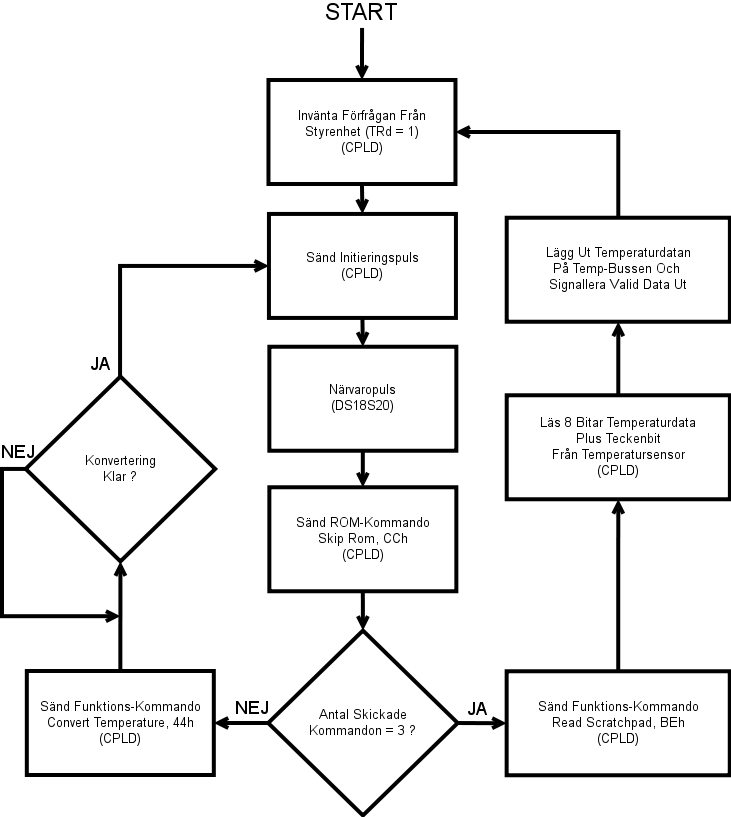
\includegraphics[scale=0.5, angle=0]{ReadCycleFlowChart.png}
		  	\caption{Högnivå-flödesdiagram för temperaturläscykel}
			\label{fig:RCFlowChart}
		\end{figure}

	\subsubsection{Uppbyggnad}

	Temperaturmodulen är baserad på en tillståndsmaskin, understödd av en intern buffer/multiplexer (MUX) samt 
	ett antal interna räknare för att generera de nödvändiga tidsfördröjningspulserna. För en grafisk beskrivning av den interna tillståndsmaskinen som används av temperaturmodulen,
	se sektion~\ref{sec:Tillstandsmaskiner}~\nameref{sec:Tillstandsmaskiner}.

	\subsubsection{Buffer/MUX}

	Buffern är en ``tri-state-buffer'' med en ``enable''-signal.
	Buffer/MUX-modulen är direkt ansluten till de två DS18S20-temperatursensorerna som använder entrådsbusskommunikationen.
	Multiplexern används för att välja mellan vilken av de två sensorerna som styrenheten vill kommunicera med.

	\subsubsection{Räknare}
	
	Internt använder temperaturmodulen ett antal räknare för att generera de nödvändiga timingpulserna och generera korrekta läs- och skrivluckor, se tabell~\ref{tab:cntTabell}.

	\begin{table} [H]
		
		\caption{Interna räknare, temperaturmodul} 
		\label{tab:cntTabell}
	\begin{tabular}{l l l}
		
		{\bf Räknare}
		\\{Namn} & {Bitar} & {Beskrivning}\\
		\hline
			cntInt & 9 & Genererar timing-pulser\\
			ZC & 4 & Hanterar timing för skriv-luckor\\
			Progress & 2 & Anger aktuellt kommando (0-3)\\
			bitCnt & 8 & Anger aktuell bit för överföring/läsning\\
	\end{tabular}
	\end{table}

	Se även VHDL-beskrivning i Appendix~\ref{sec:programlistningar}. \\

	\subsection{Extern funktionsstyrning}

Funktionsmodulen tar emot data från styrenheten och skickar vidare 
uppdateringarna på funktionsutgångarna som används för funktionerna. Sammanfattat fungerar den som ett
mellansteg för att underlätta för styrenhetens funktionsutgångsstyrning, och kan vid behov byggas ut ytterligare
för att implementera andra funktioner i systemet.

	\subsection{Användargränssnittshantering}

Systemet har, förutom DTMF-kontroll, även ett lokalt knappsatsgränssnitt och en till/från-brytare för temperaturläsning.
Dessa rådata måste formateras, avkodas och presenteras för styrenheten. Detta är knappsatsmodulens uppgift.

Om en knapp på knappsatsen trycks ned, skickas en ``available''-signal (dAv) från knappsatsen till knappsatsmodulen, som sedan
avkodar vilken knapp som tryckts ned, och presenterar detta för styrenheten genom att höja en ``keyboard available'' (kAv)-signal,
vilket indikerar giltig data på knappsatsdatabussen (kData[3..0]). Genom att skicka en ``acknowledgement''-signal (kAck) bekräftar 
styrenheten att den sett och mottagit datan från knappsatsen.

\section{Hårdvara}

Nedan presenteras hårdvaran som systemet är uppbyggt av, under respektive rubrik. Se även komponentlista i tabell~\ref{tab:komponentlista}, Appendix~\ref{sec:komponentlistasec}
samt kretsschema i figur~\ref{fig:schema} , Appendix~\ref{sec:kretsschema}. Pinlayouten för CPLD-kretsarna ges i kretsschemat.

\label{hårdvara}
	\subsection{ISD2560P}
	\label{ISD2560P}
ISD2560P är en integrerad inspelnings- och uppspelningskrets från Futurlec, med plats för 60 sekunder ljud. Kretsen är inkopplad enligt ett modifierat förslagsschema i databladet och brukas i ``Direct Addressing Mode''. Kretsen adresseras med 10 bitar, vilket ger 600 giltiga adresser. Varje adressinkrementering flyttar uppspelningspekaren med 0.1 sekunder ($0.1 $ sekunder $* 600$ adresser $= 60$ sekunder). Signalerna ``chip enable'' (ce), ``end of message'' (eom) och en 6-bitars adressbuss är anslutna till CPLDn. Uppspelningen styrs av den flanktriggade signalen ce som är aktiv låg. När denna får en puls latchas adressvärdena och en uppspelning påbörjas. Uppspelning avslutas med en annan (aktiv låg) puls på eom.

De 3 minst signifikanta adressbitarna och den mest signifikanta adressbiten är knutna till jord. Resterande 6 bitar styrs av CPLDn. Inkoppling på detta vis innebär ljudklippslängder i multiplar av 0.8 sekunder. Alla siffror som läses upp ryms i enskilda 0.8-sekundersblock och kan således adresseras utan vidare. Längre ljudklipp kräver aldrig mer än 1.6 sekunder och kan tilldelas block av dubbel längd genom att använda 5-bitarsadressering med en statisk LSB.
	Se även datablad i Appendix~\ref{sec:datablad}.

	\subsection{DS18S20}
	\label{DS18S20}
		Den temperatursensor som används är Maxim DS18S20, som ger temperaturmodulen möjlighet att läsa av temperaturen
		med nio bitars upplösning. Sensorerna som används i detta system drivs av en extern spänningskälla på +5V,
		och kommunicerar seriellt över en entrådsbuss. Seriekommunikationen baseras på att ``bus-mastern'' (med bus-mastern avses här CPLD1) initierar skriv-
		och läsluckor. Mellan varje skriv- eller läslucka finns en kort återhämtningsperiod. Temperatursensorn initieras genom att mastern
		driver bussen låg, vilket följs av att temperatursensorkretsen driver för att signalera närvaro.
		Efter initieringen väntar sensorkretsen på ett ROM-kommando från mastern,
		följt av ett funktionskommando. Varje sådant kommando är en byte långt och skickas som LSB-först. Mastern skickar
		en logisk nolla genom att driva bussen låg under hela skrivluckan. En etta skickas genom att mastern driver bussen låg
		under en kort del av skrivluckan och sedan släpper bussen under resten av skrivluckans längd. 

		Då mastern är klar med att skicka över ROM- och funktionskommando, kan (beroende på vilka kommandon som sändes) DS18S20-kretsen
		svara med aktuell data. På samma sätt som ovan måste mastern här initiera en läslucka. 
		DS18S20-kretsen svarar på den allokerade läsluckan och överför etta eller nolla. Mastern kan då sampla bussen för att läsa av vad DS18S20-kretsen skickat. All data från
		temperatursensorn skickas som ``LSB-first'' och i 2-komplementsform. För exakta tidskrav, se datablad i Appendix~\ref{sec:datablad}

	\subsection{MT8880C}
	\label{MT8880C}
		Avkodning av inkommande DTMF-signaler avkodas med hjälp av MT8880C från Mitel. 
		Telefonsignalen kopplas direkt in till DTMF-överföraren enligt specifikation för standarduppkoppling i datablad. Endast avkodningsfunktionen på 		kretsen används. Databuss, r/w-signal, irq och $\Phi$2 är anslutna till styrenheten. 
		``chip select'' (ce) är satt konstant låg då denna krets använder bussen exklusivt. 
Före initiering skickas manuellt en initieringssekvens till kretsen minst $100 \, m s$ efter spänningspåslag. Detaljer om initieringscykeln finns i databladet för MT8880C, se Appendix~\ref{sec:datablad}.

\section{Tillståndsmaskiner}

	Nedan beskrivs modulernas tillståndsmaskiner. Varje tillståndsmaskin presenteras
	som en lista över tillstånd med förklaringar, samt som ett grafiskt tillståndsdiagram.
	Diagrammen är uppbyggda enligt principen som visas i figur~\ref{fig:SMExp}\\
	
	\begin{figure}[H]
	  \centering
	      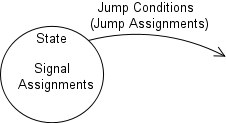
\includegraphics[scale=0.5, angle=0]{StateMachineExplained.png}		
	  	\caption{Förklaring till tillståndsdiagram}	
		\label{fig:SMExp}
	\end{figure}
	
\label{sec:Tillstandsmaskiner}	

\pagebreak
	
\subsection{Styrenhet}

			Se figur~\ref{fig:CUSM}\\
			{\bf Reset:} Alla signaler sätts låga.\\
			{\bf Grundvärden:} Utgångspunkten är att alla signaler behåller sina gamla värden om inget annat anges.\\
			\begin{tabular}{l}
				\\{\bf Viloläge (tillstånd 0):}\\
				0: Inväntar samtal.\\
				{\bf Temperaturuppläsning (tillstånd 1-5):}\\
				3: Läser upp ljud ``Temperaturen inne är''.\\
				4: Läser upp innetemperatur.\\
				3: Läser upp ljud ``Temperaturen ute är''.\\
				4: Läser upp utetemperatur.\\
				5: Läser upp ljud ``Funktionskommandotilldelning''.\\
				{\bf Kommando (tillstånd 6):}\\
				6: Inväntar funktionskommando eller avslutat samtal.\\
				{\bf Funktionstilldelning (Tillstånd 7-11):}.\\
				7: Uppdaterar/läser upp funktionsstatus för funktion 1.\\
				8: Uppdaterar/läser upp funktionsstatus för funktion 2.\\
				9: Uppdaterar/läser upp funktionsstatus för funktion 3.\\
				10: Uppdaterar/läser upp funktionsstatus för funktion 4.\\
				11: Läser upp funktionsstatus ``till/från''.\\
			\end{tabular}

	\begin{figure}[H]
	  \centering
	      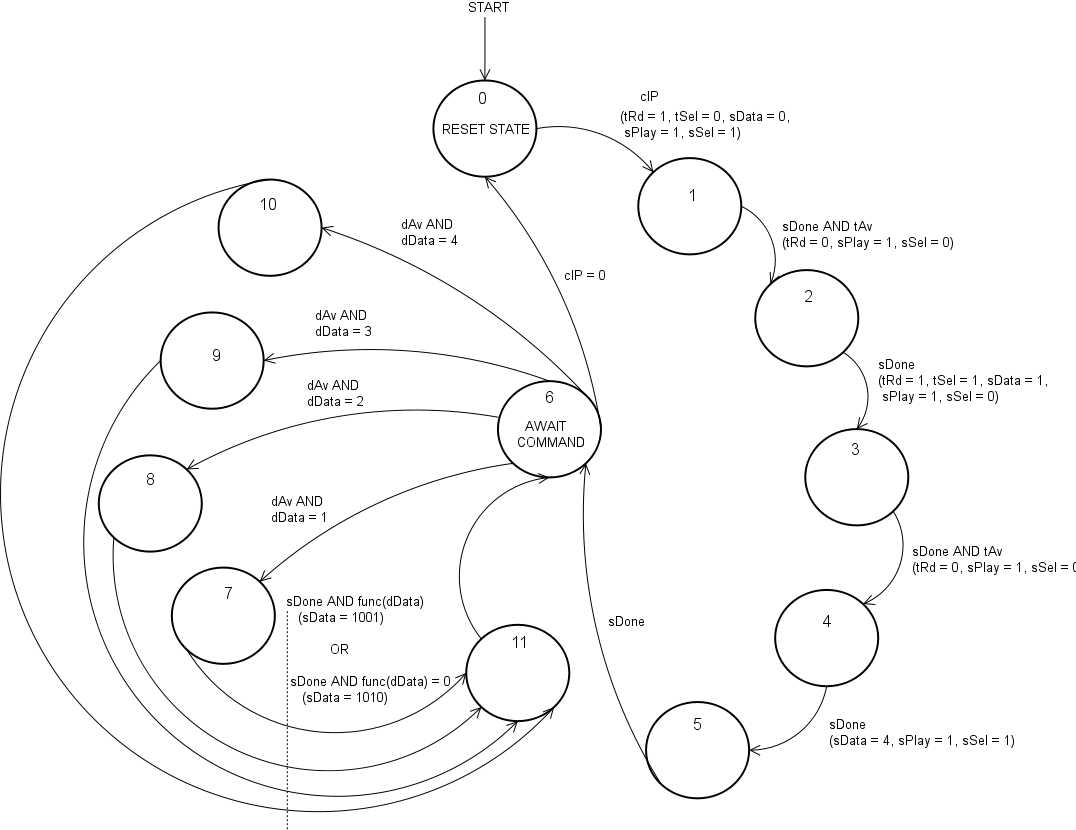
\includegraphics[scale=0.4, angle=0]{ControlUnitStateMachineDiagram.png}
	  	\caption{State machine-diagram för styrenhet}
		\label{fig:CUSM}
	\end{figure}
	
	\pagebreak

		\subsection{Temperaturmodul}
			Se figur~\ref{fig:TempSM}.\\
			{\bf Reset:} Alla signaler och räknare sätts låga.\\
			{\bf Grundvärden:} Utgångspunkten är att alla signaler behåller sina gamla värden om inget annat anges.\\
			\begin{tabular}{l}
				\\{\bf Viloläge (tillstånd 0):}\\
				0: Viloläge och återställningspunkt. inväntar tRd från styrenheten.\\
				{\bf Initialisering (tillstånd 1-3):}\\
				1: Fördröjningstillstånd, väntar på puls på delayLong ($512 \, \mu s$).\\
				2: Mastern driver bussen låg i $512 \, \mu s$ och sätter datavärdet till 0xCC (Skip ROM).\\
				3: Mastern släpper bussen, DS18S20 skickar närvaropuls.\\
				{\bf Kommandoöverföring (tillstånd 4-8):}\\
				4: Förberedelsetillstånd före sändning.\\
				5: Huvudsändningstillståndet, mastern sänder bit enligt aktuellt räknarvärde.\\
				6: Mellanbittillstånd, återhämtningstillständ. Fortsätter om fler bitar ska skickas.\\
				7: Avgör om DS18S20 är upptagen med att konvertera temperaturen. Om så, vänta tills klar.\\
				8: Vägskälstillstånd. Om fler kommandon kvar att skicka, gå tillbaka, annars börja läsa.\\
				{\bf Läsning (Tillstånd 9-15):}.\\
				9:  Förberedelsetillstånd före läsning.\\
				10: Mastern initierar en läslucka genom att dra bussen låg i $4 \, \mu s$.\\
				11: Mastern väntar ytterligare $4 \, \mu s$ för att pull-up-motståndet ska få verka.\\
				12: Mastern samplar bussen. Om DS18S20 skickar en nolla hålls bussen låg, annars inte.\\
				13: Återhämtningstillstånd mellan samplingar.\\
				14: Vägskälstillstånd. Om vi har fler bitar att läsa, gå tillbaka, annars gå vidare.\\
				15: Läsning klar, lägg ut temperatur på buss och signalera giltig data. Gå tillbaka till 0.\\
			\end{tabular}

	\begin{figure}[H]
	  \centering
	      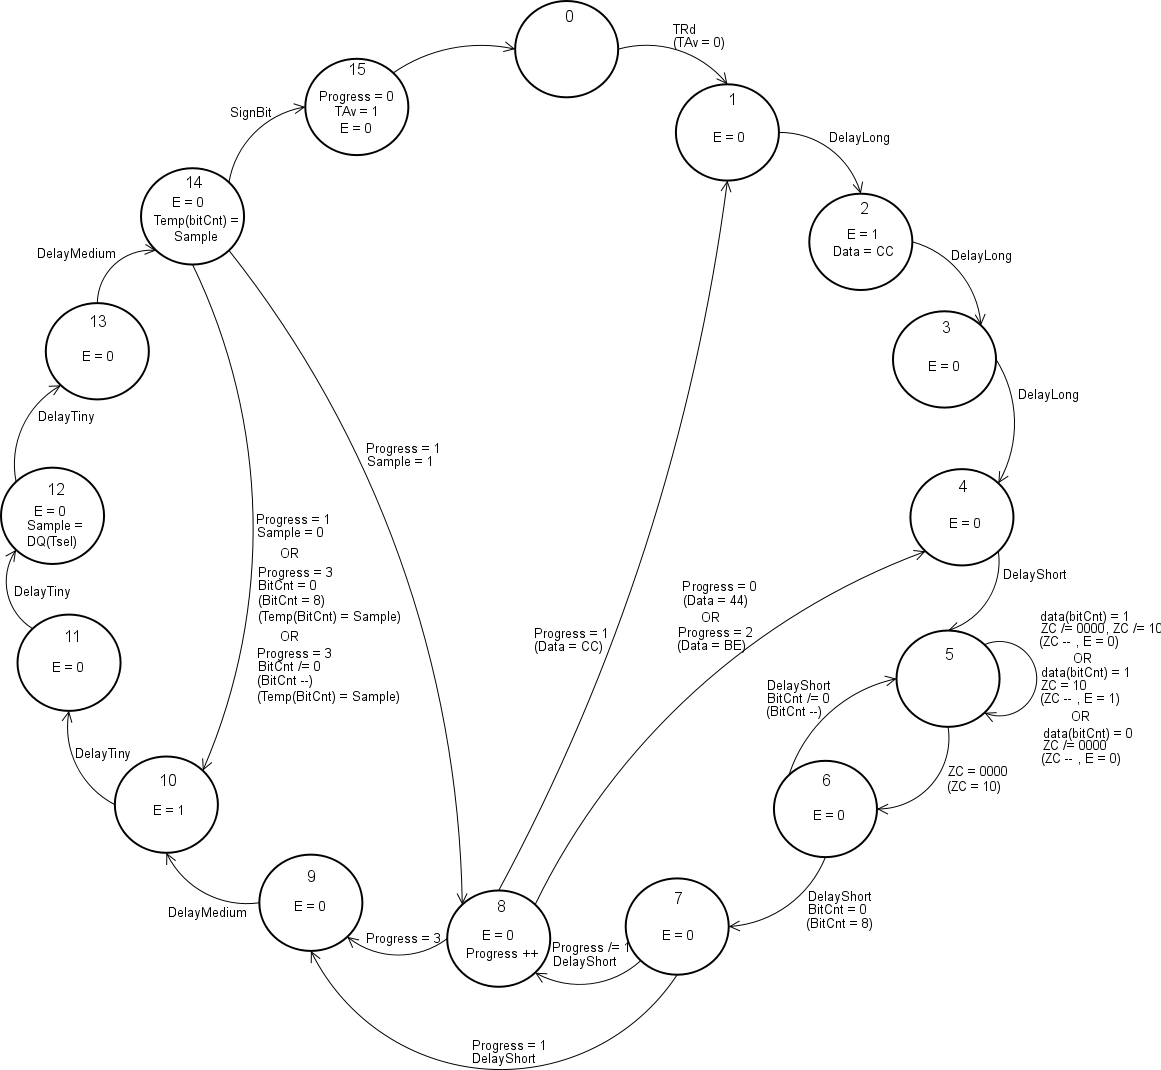
\includegraphics[scale=0.4, angle=0]{TempStateMachineDiagram.png}
	  	\caption{Detaljerat state machine-diagram för temperaturläscykel}
		\label{fig:TempSM}
	\end{figure}
	
\pagebreak

		\subsection{DTMF-Modul}

			Se figur~\ref{fig:DTMFSM}.\\
			{\bf Reset:} Alla signaler sätts låga.\\
			{\bf Grundvärden:} Utgångspunkten är att alla signaler är satta till 0 om inget annat anges.\\
			\begin{tabular}{l}
				\\{\bf Viloläge (tillstånd 0):}\\
				0: Viloläge och återställningspunkt, inväntar ``sigInit''.\\
				{\bf Initialisering (tillstånd 1-20):}\\
				1-3: Läs statusregister.\\
				4-6: Skriver `0000' till kontrollregister A.\\
				7-8: Skriver `0000' till kontrollregister A.\\
				9-11: Skriver `1000' till kontrollregister A.\\
				12-14: Skriver `0000' till kontrollregister B.\\
				15-17: Läser statusregister.\\
				18-20: Intialisering av Chip-interface.\\
				{\bf Läsning (Tillstånd 21-26):}\\
				21:  Viloläge, inväntar giltig data från MT8880C.\\
				22-23:  Läs data från MT8880C.\\
				24-25:  Lägg ut data på intern databuss och signalera giltig data.\\
				26:  Inväntar bekräftelsesignal från styrenhet.\\				
			\end{tabular}

	\begin{figure}[H]
	  \centering
	      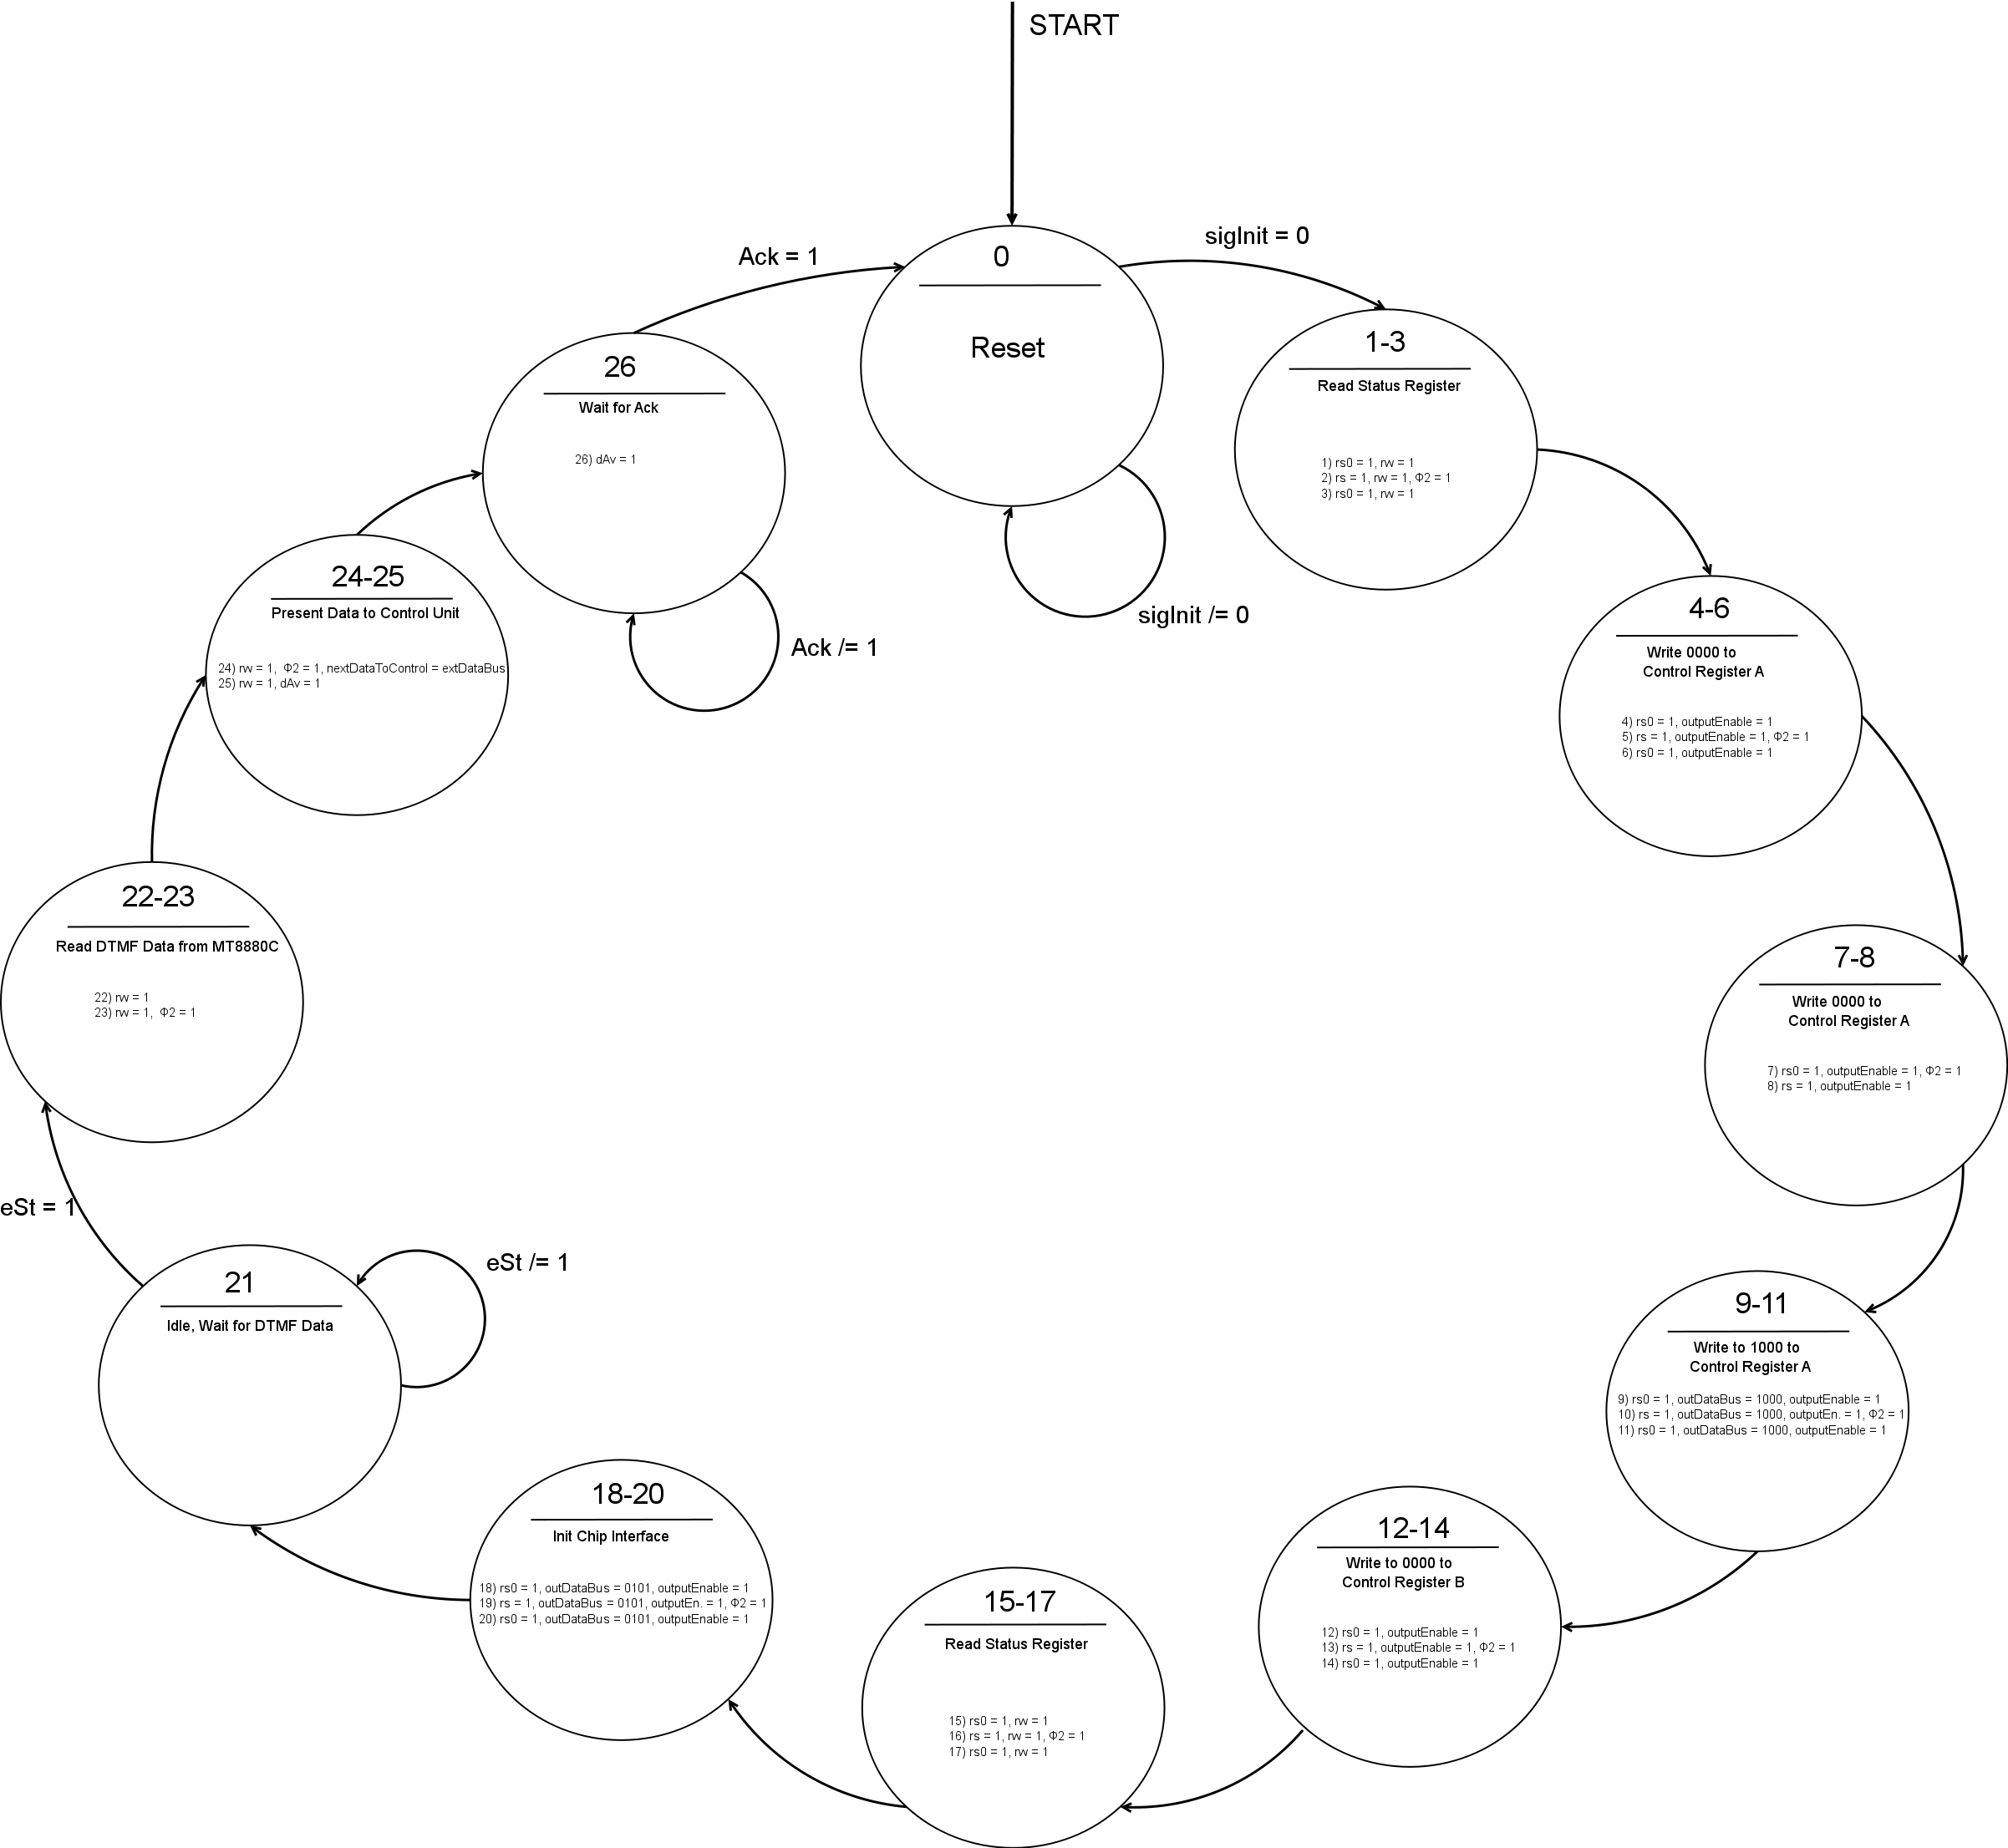
\includegraphics[scale=0.18, angle=0]{DTMFStateMachineDiagram.png}		
	  	\caption{Förenklat state machine-diagram för DTMF-Modul}
		\label{fig:DTMFSM}
	\end{figure}
	
\pagebreak

		\subsection{Ljudmodul}

			Se figur~\ref{fig:SoundSM}\\
			{\bf Reset:} Alla signaler återställs låga.\\
			{\bf Grundvärden:} Alla signaler låga, utom ce som är hög.\\
			\begin{tabular}{l}
				\\{\bf Viloläge (tillstånd S0):}\\
				S0: Inväntar play-signal.\\
				{\bf Spela upp Ljud (C)}\\
				S1C: Sätt adress.\\
				S2C: Spela upp ljud, vänta tills uppspelning är klar.\\
				S3C: Signalera uppspelning klar till styrenhet.\\
				{\bf Spela upp Temperatur}\\
				S1T: Sätt adress.\\
				S2T: Spela upp temperatur, vänta tills uppspelning klar.\\
				{\bf Spela upp Temperatur (vid overflow)}\\
				S1TO: Sätt adress.\\
				S2TO: Spela upp temperatur, vänta tills uppspelning klar.\\
				{\bf Spela upp Positiv/Negativ}\\
				S3TP: Sätt adress (positiv temperatur).\\
				S3TM: Sätt adress (negativ temperatur).\\
				S4TP: Spela upp positiv, vänta tills klar.\\
				S3TM: Spela upp negativ, vänta tills klar.\\
			\end{tabular}

	\begin{figure}[H]
	  \centering
	      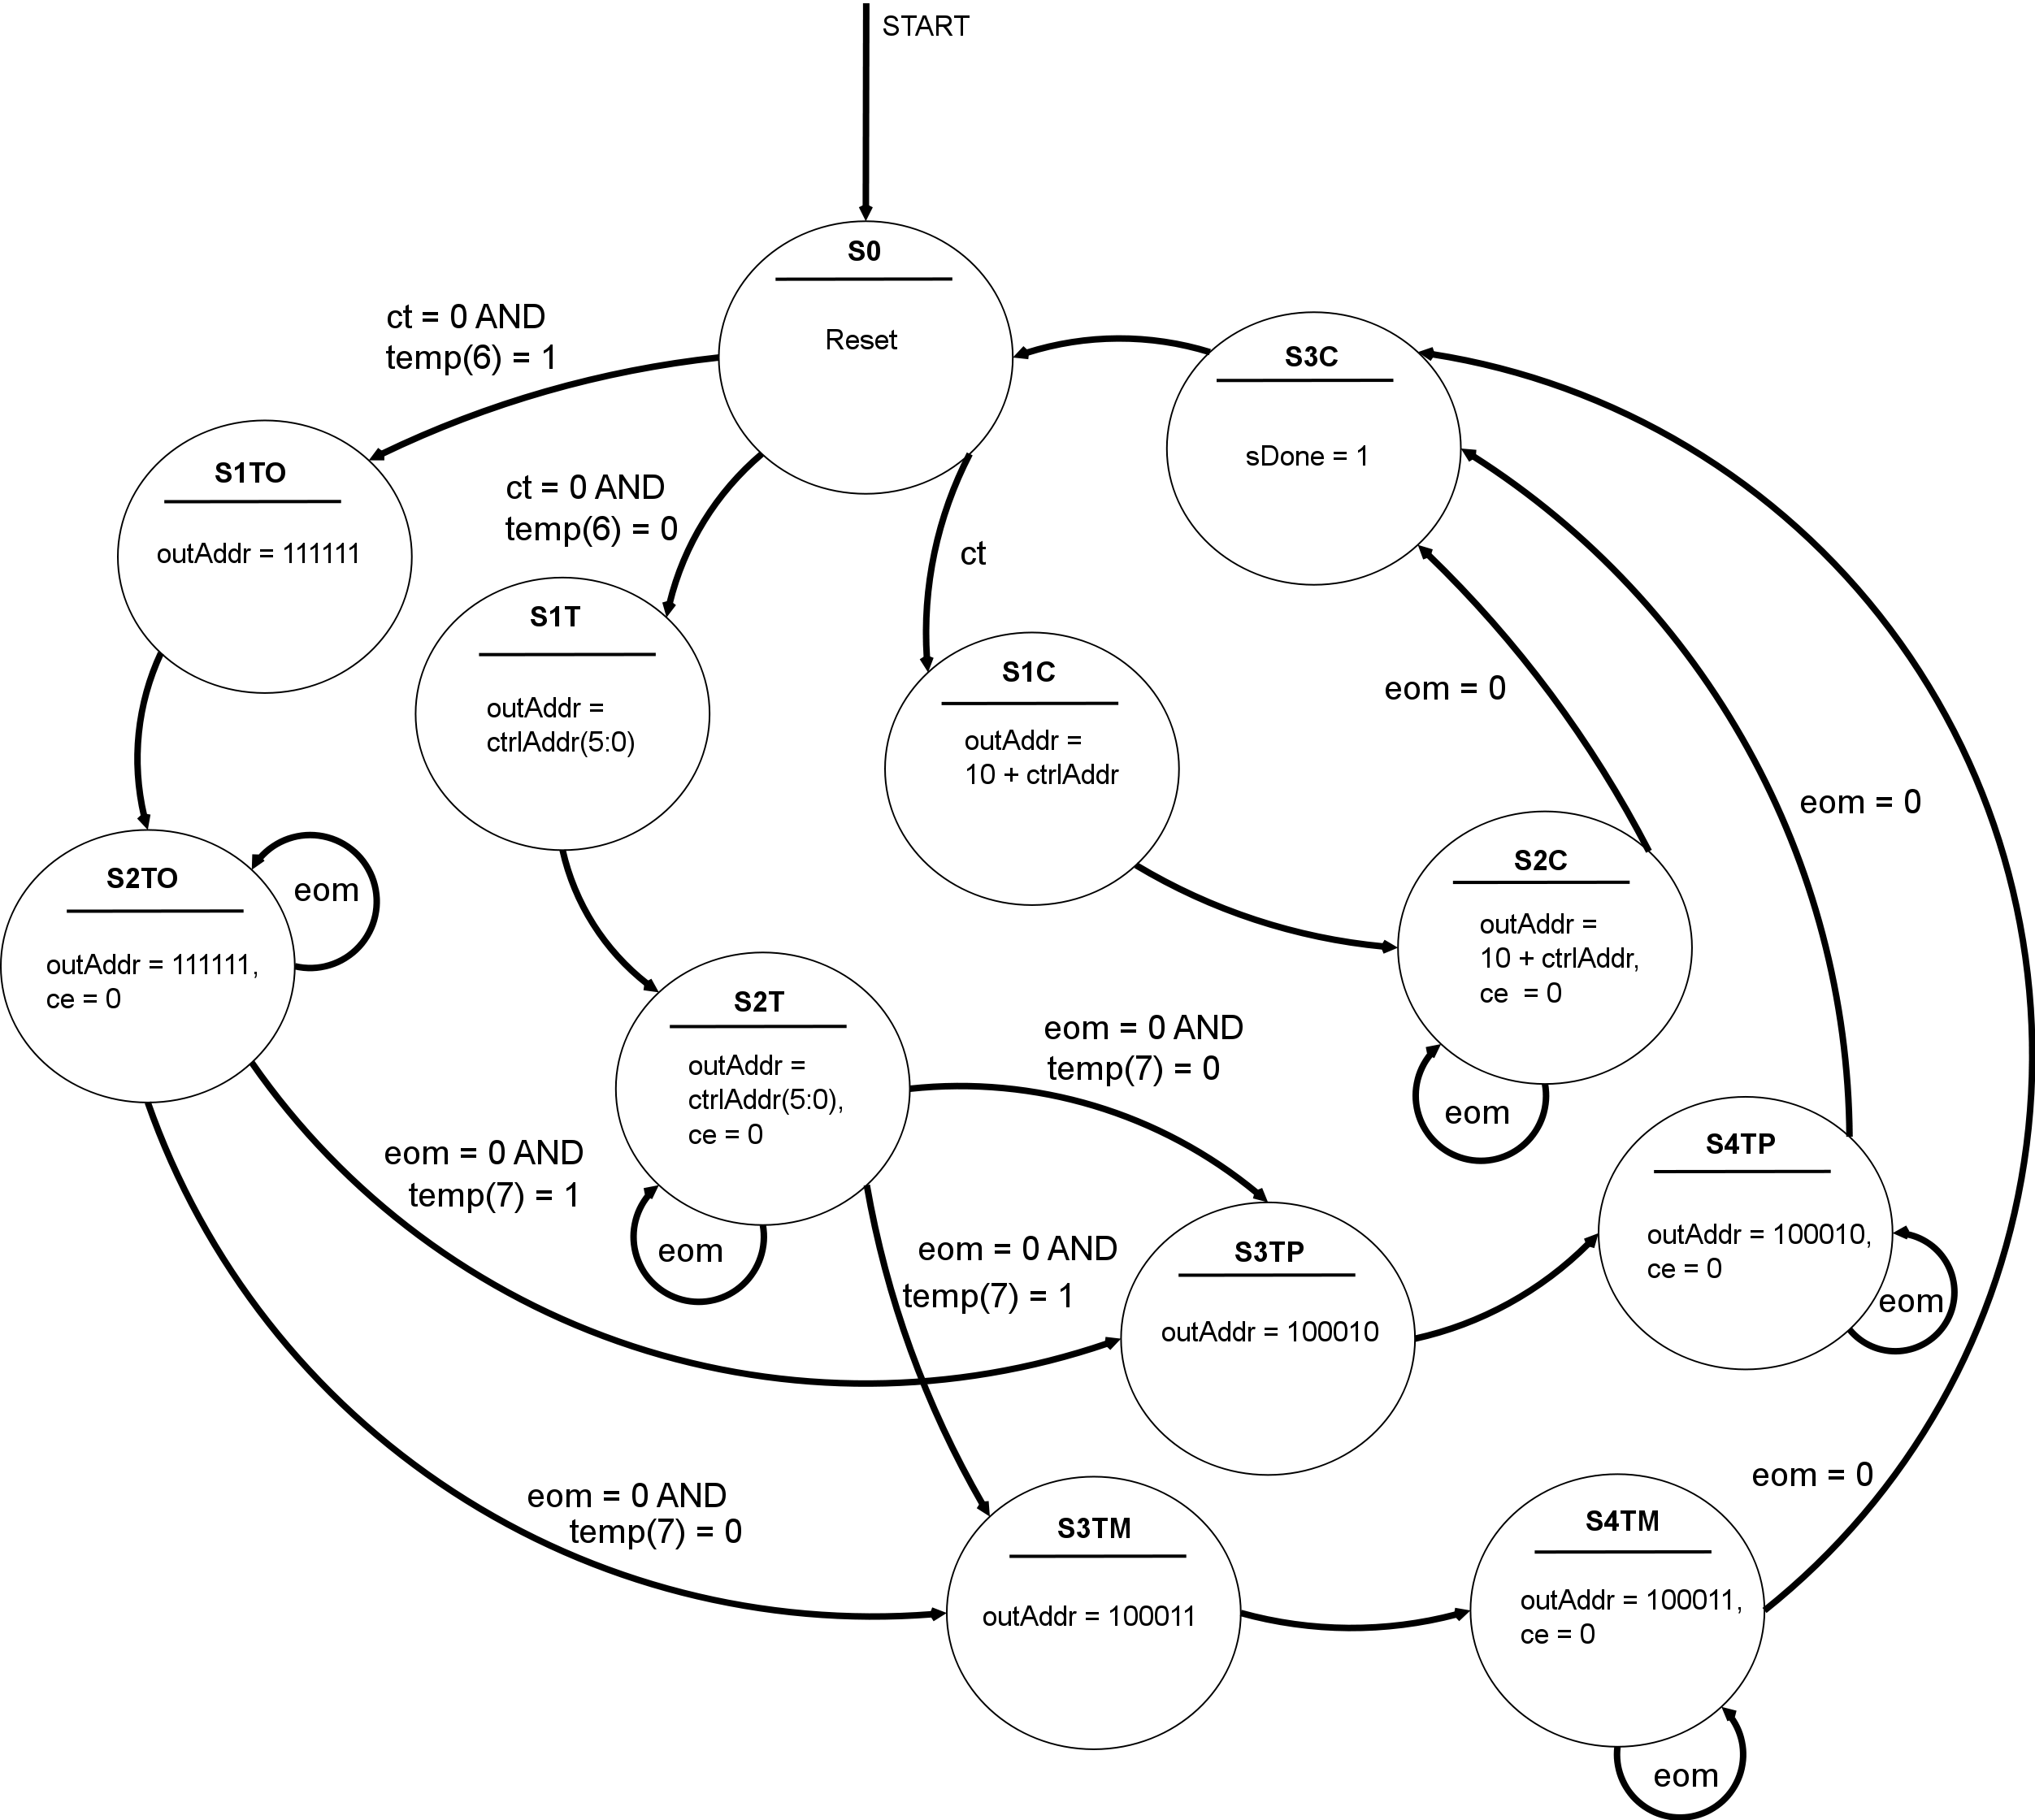
\includegraphics[scale=0.18, angle=0]{SoundStateMachineDiagram.png}
	  	\caption{State machine-diagram för ljudenhet}
		\label{fig:SoundSM}
	\end{figure}

\pagebreak

\section{Felanalys}

Då systemet hanterar avläsning av temperaturer och endast klarar ett begränsat temperaturintevall
görs här en felanalys. För de tillämpningsområden systemet är konstruerat för (hemanvändare) 
är mätfelen dock för små för att ha betydelse; noggrannheten är större än vad behovet åkallar.

Temperatursensorerna arbetar med en temperaturupplösning på $0,5\,^{\circ}\mathrm{C}$ enligt datablad, se Appendix~\ref{sec:datablad}. Temperaturen levereras på en absolut skala och sensorerna ska leverera en exakthet på $\pm 0,5\,^{\circ}\mathrm{C}$ i intervallet $-10\,^{\circ}\mathrm{C}$ till $+85\,^{\circ}\mathrm{C}$. Resultatet som presenteras på LED-displayen är hela det avlästa värdet i binär form, medan ljuduppspelningen inte presenterar mer än en grads upplösning.
Systemet arbetar med ett temperaturspann på $\pm 32\,^{\circ}\mathrm{C}$. Temperaturer utanför intervallet representeras som högsta respektive lägsta värde.

\pagebreak

	\appendix
	\renewcommand{\appendixpagename}{Appendix}
	\appendixpage
	\renewcommand{\appendixtocname}{Appendix}

	\addappheadtotoc

	\section{Användarmanual och Gränssnitt}
	\label{sec:Manual}
	För att använda systemet, spänningssätt $+5V$ DC mellan ingångarna ``+5V'' och ``GND'' och koppla in telefonlinje till DTMF-anslutningen.
	När systemet är startat ska det återställas (röd tryckknapp) och sedan initieras (svart tryckknapp).
	Efter detta är systemet redo att användas, kommando kan ges via telefon eller manuell knappsats, se figur~\ref{fig:UserInterface}.
	När som helst kan systemet startas om helt genom att igen trycka på den röda tryckknappen. Det finns även en knapp för
	att slå till eller från kontinuerlig avläsning av temperatur.
	Då systemet blir uppringt läses temperaturen upp, sedan kan kommandon ges från användaren enligt nedan:\\

	\begin{table}[ht]
		\begin{minipage}[b]{0.5\linewidth}\centering
			{\bf Knappsats}\\
			\begin{tabular}{l c r}
				\\{\bf Knapp} & {\bf Funktion}\\
				1 & Funktion 1 TILL\\		
				2 & Funktion 2 TILL\\		
				3 & Funktion 3 TILL\\
				4 & Funktion 1 FRÅN\\	
				5 & Funktion 2 FRÅN\\
				6 & Funktion 3 FRÅN\\		
				A & Visa Innetemperatur\\
				B & Visa Utetemperatur \\\\
			\end{tabular}
	 	\end{minipage}
	 	\hspace{0.5cm}
	 	\begin{minipage}[b]{0.5\linewidth}
			\centering
			{\bf Telefon}\\
			\begin{tabular}{l c r}
				\\{\bf Knapp} & {\bf Funktion}\\
				1 & Funktion 1 TILL\\		
				2 & Funktion 2 TILL\\		
				3 & Funktion 3 TILL\\
				4 & Funktion 1 FRÅN\\	
				5 & Funktion 2 FRÅN\\
				6 & Funktion 3 FRÅN\\
				9 & Visa Innetemperatur\\
				0 & Visa Utetemperatur \\\\
			\end{tabular}
	 	\end{minipage}
	\end{table}

		\begin{figure}[H]
		  \centering
		      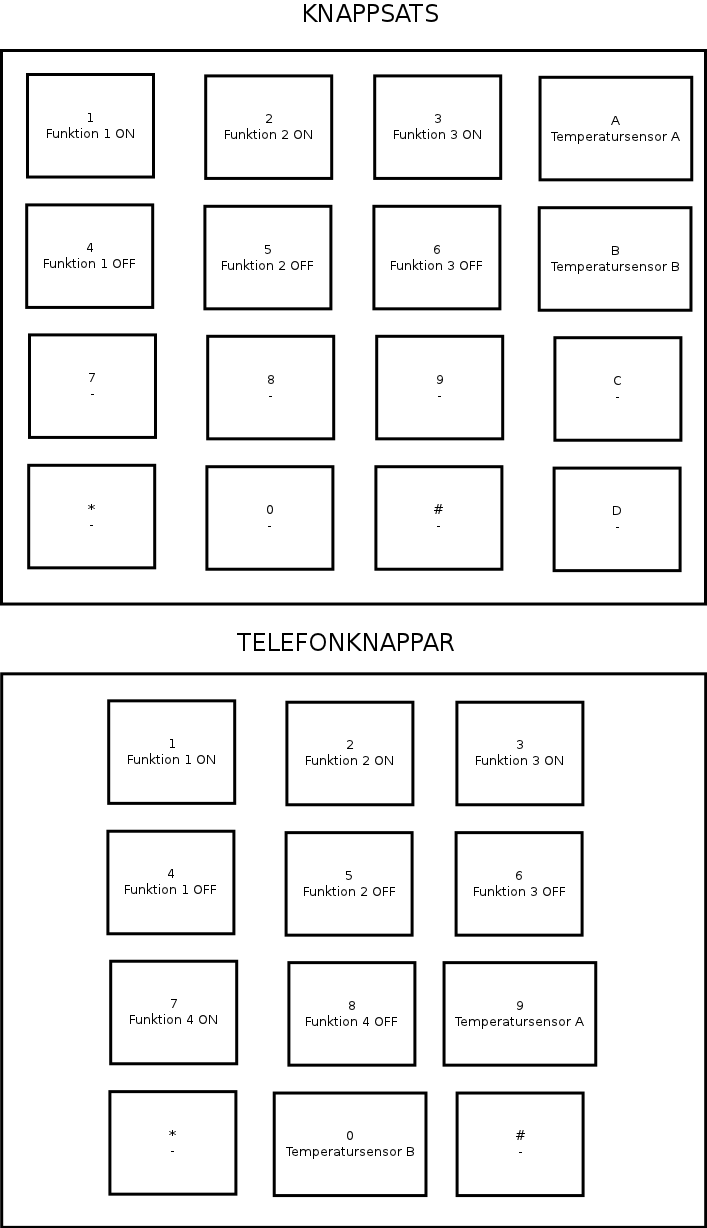
\includegraphics[scale=0.40, angle=0]{UserInterface.png}
			\label{fig:UserInterface}
		  	\caption{Knapplayout, knappsats resp. telefon}
		\end{figure}

	\section{Blockschema}
		\label{sec:BlockAppendix}
		\begin{figure}[H]
		  \centering
		      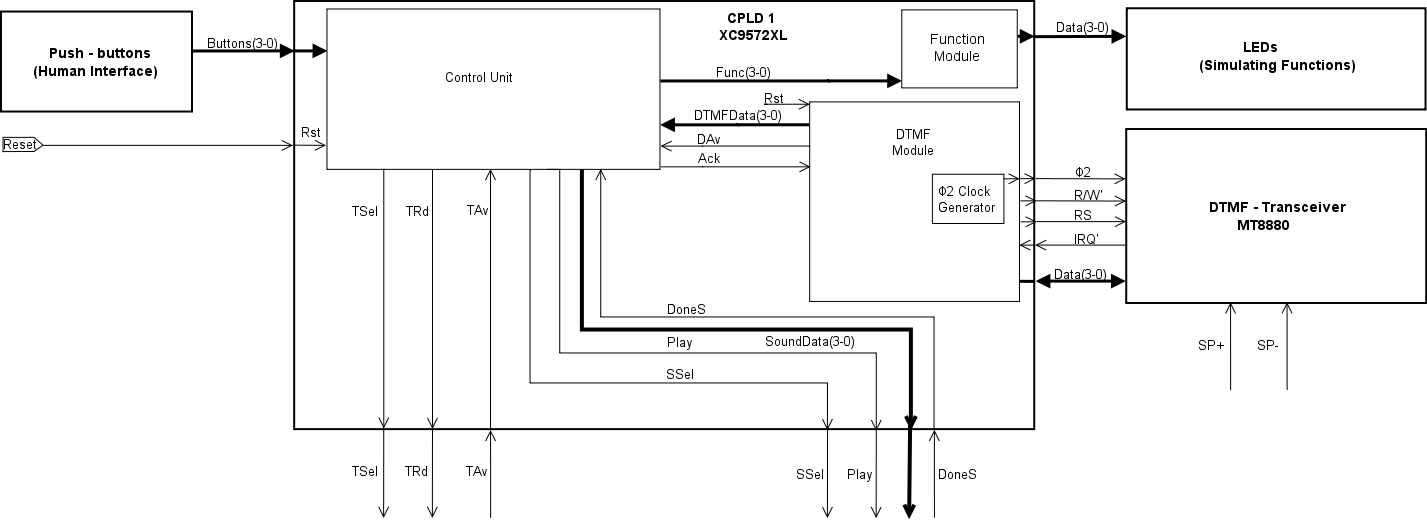
\includegraphics[scale=0.36, angle=90]{BlockDiagramCPLD1.png}
			\label{fig:BlockDiagram1}
		  	\caption{Blockschema (CPLD1)}
		\end{figure}

		\begin{figure}[H]
		  \centering
		      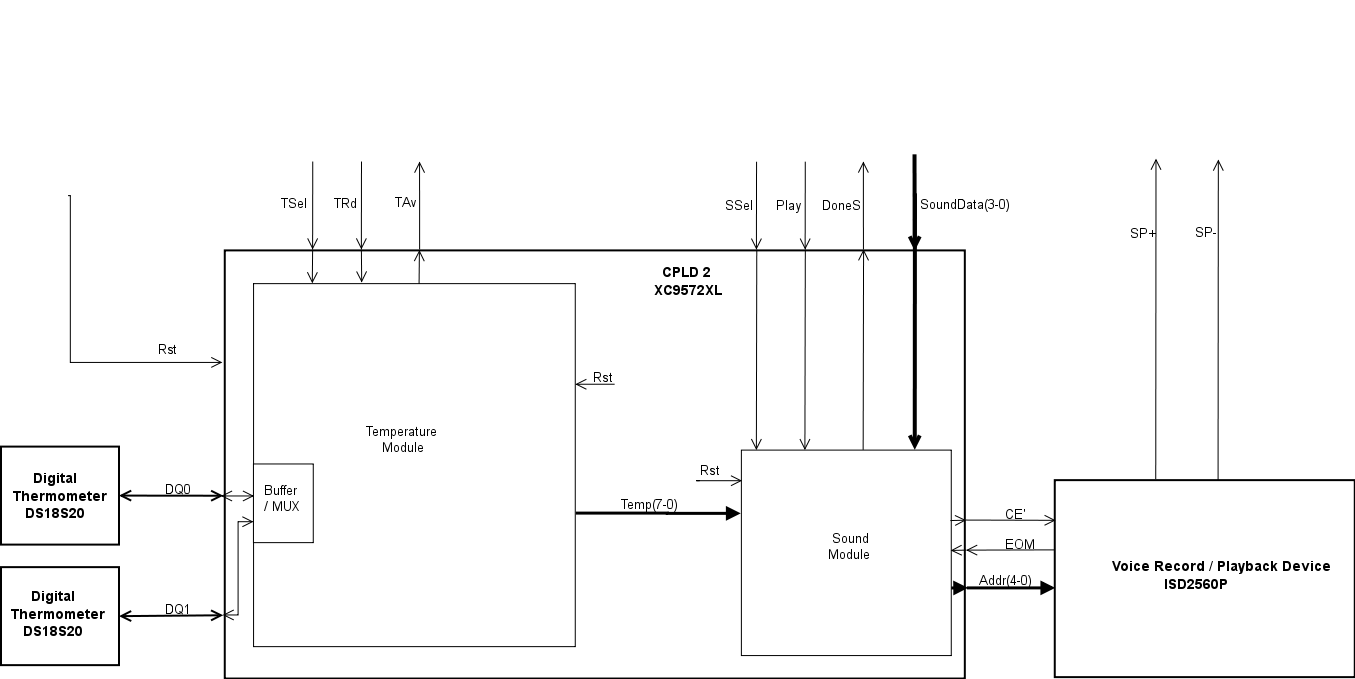
\includegraphics[scale=0.40, angle=90]{BlockDiagramCPLD2.png}
			\label{fig:BlockDiagram2}
		  	\caption{Blockschema (CPLD2)}
		\end{figure}
	
		\begin{figure}[H]
		  \centering
		      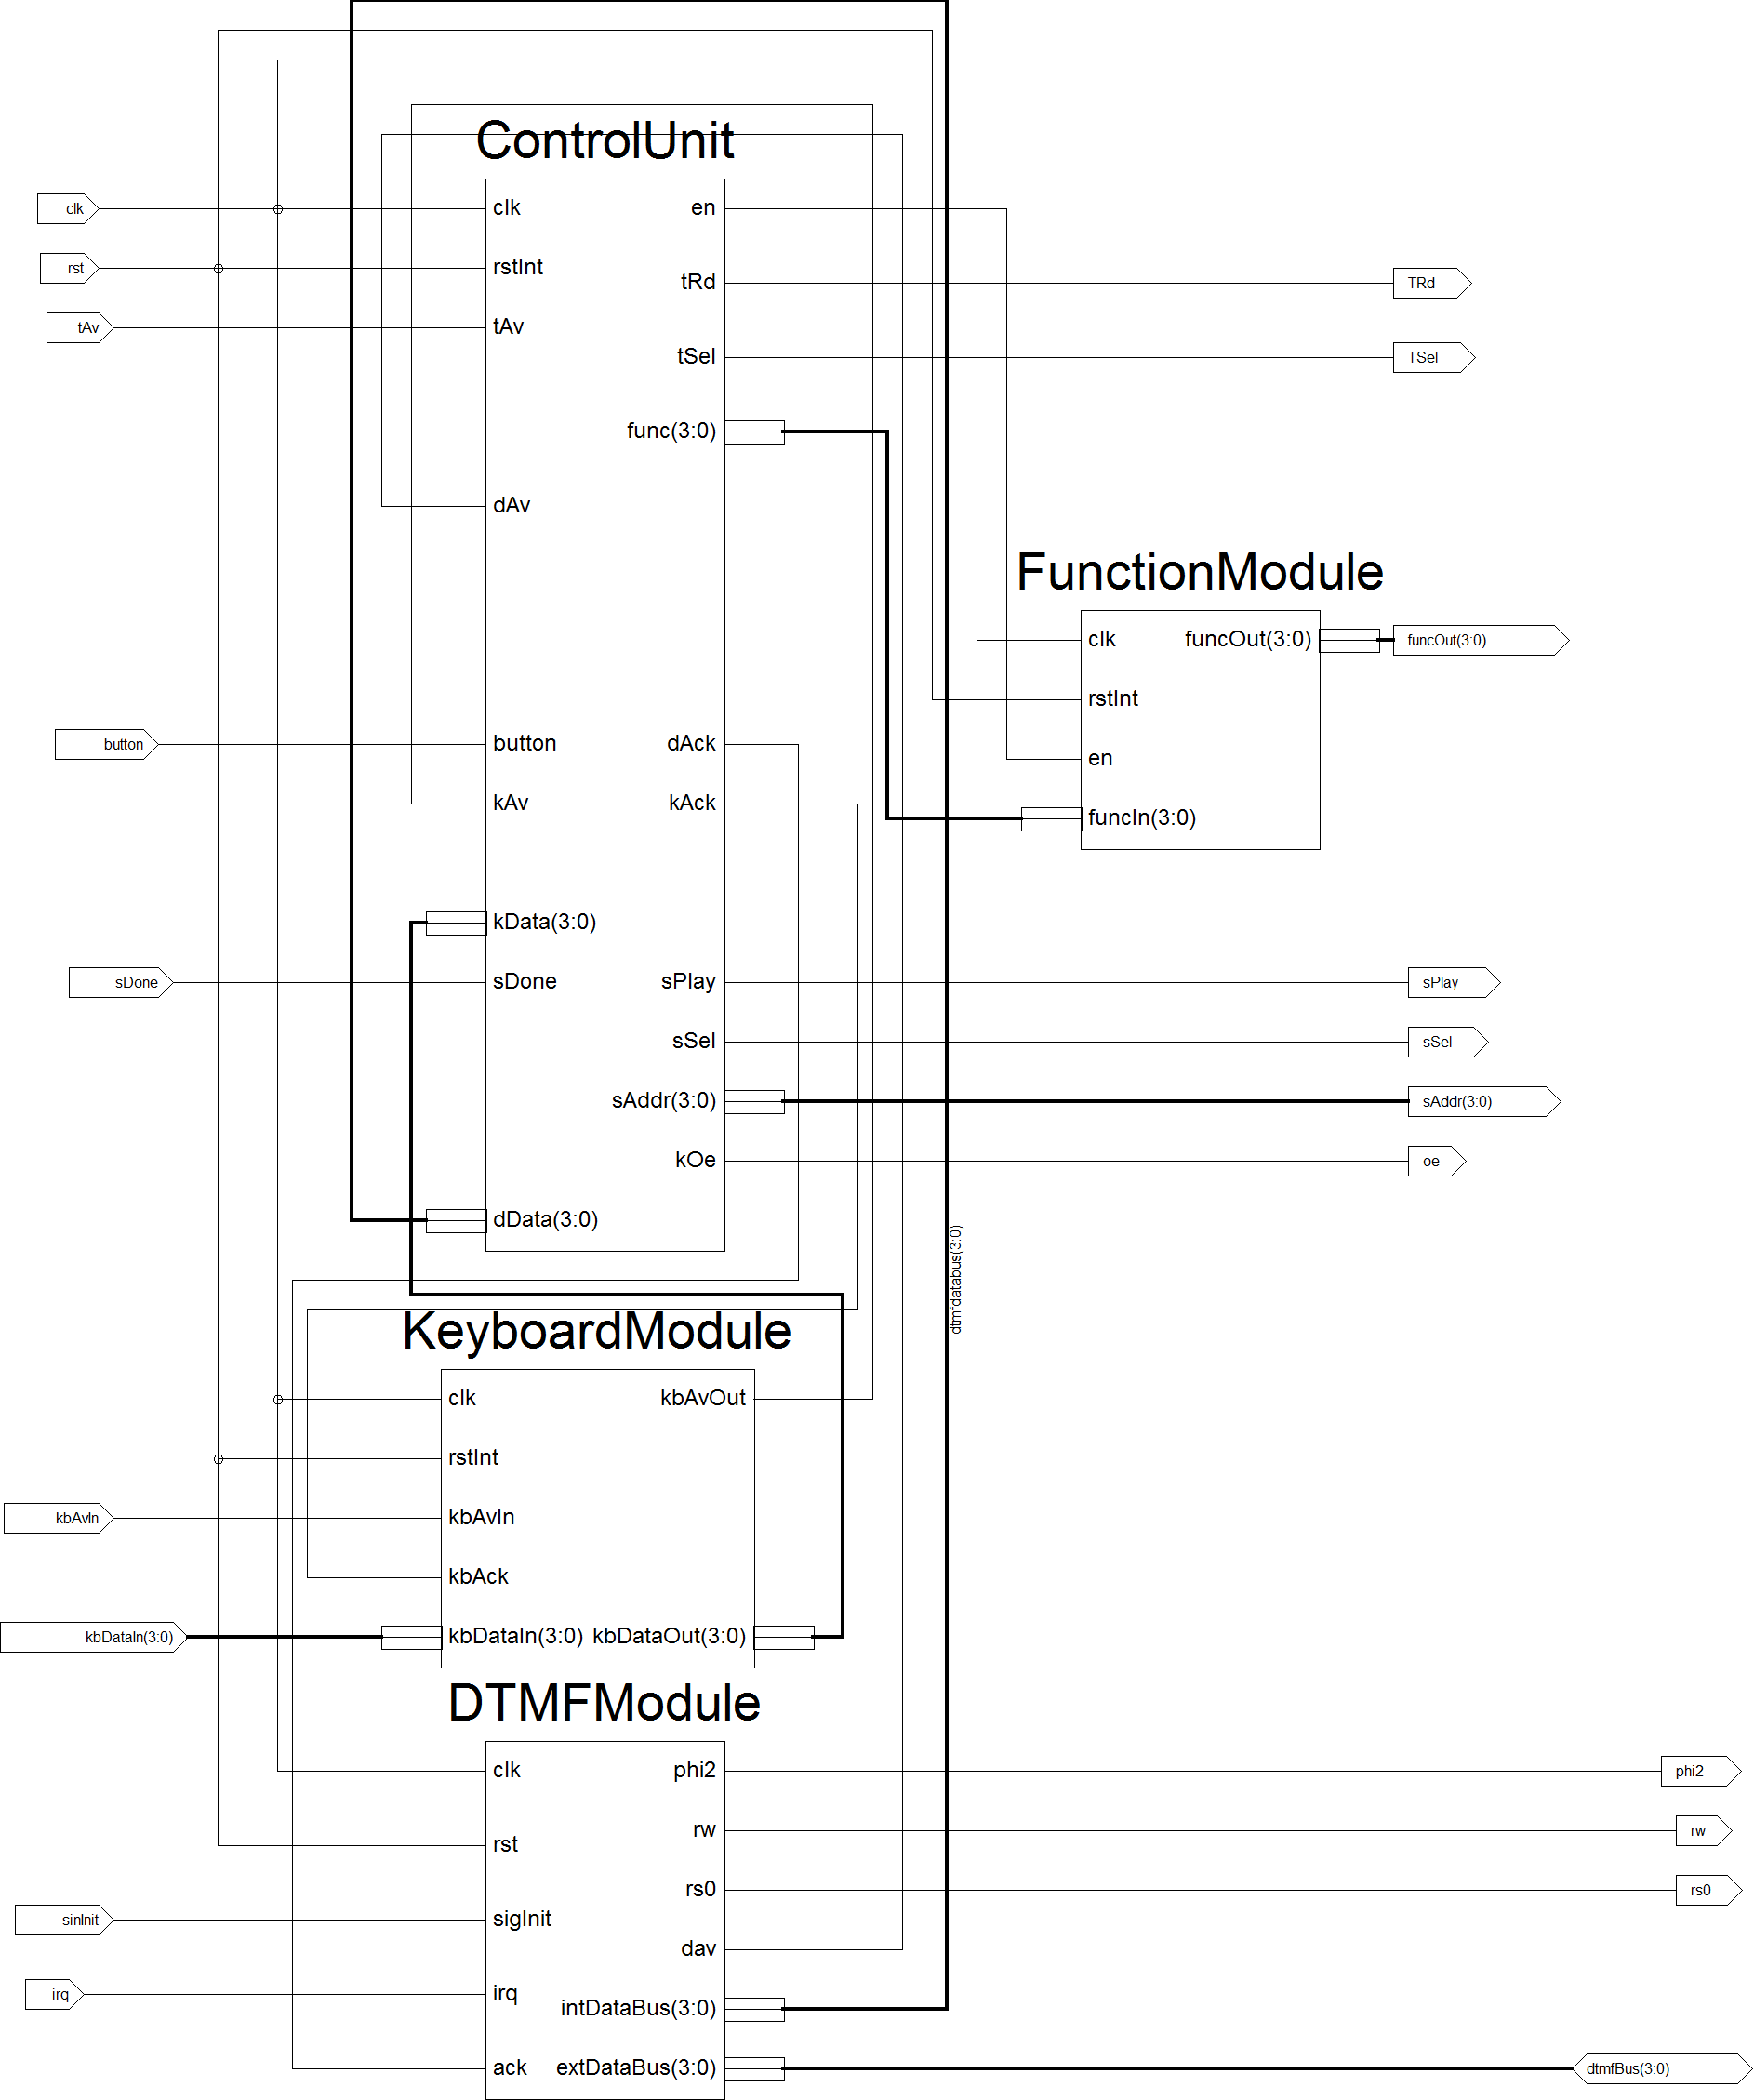
\includegraphics[scale=0.30, angle=0]{Xilinx_CPLD1.png}
			\label{fig:BlockDiagram2}
		  	\caption{Internt blockschema, moduler (CPLD1)}
		\end{figure}
	
		\begin{figure}[H]
		  \centering
		      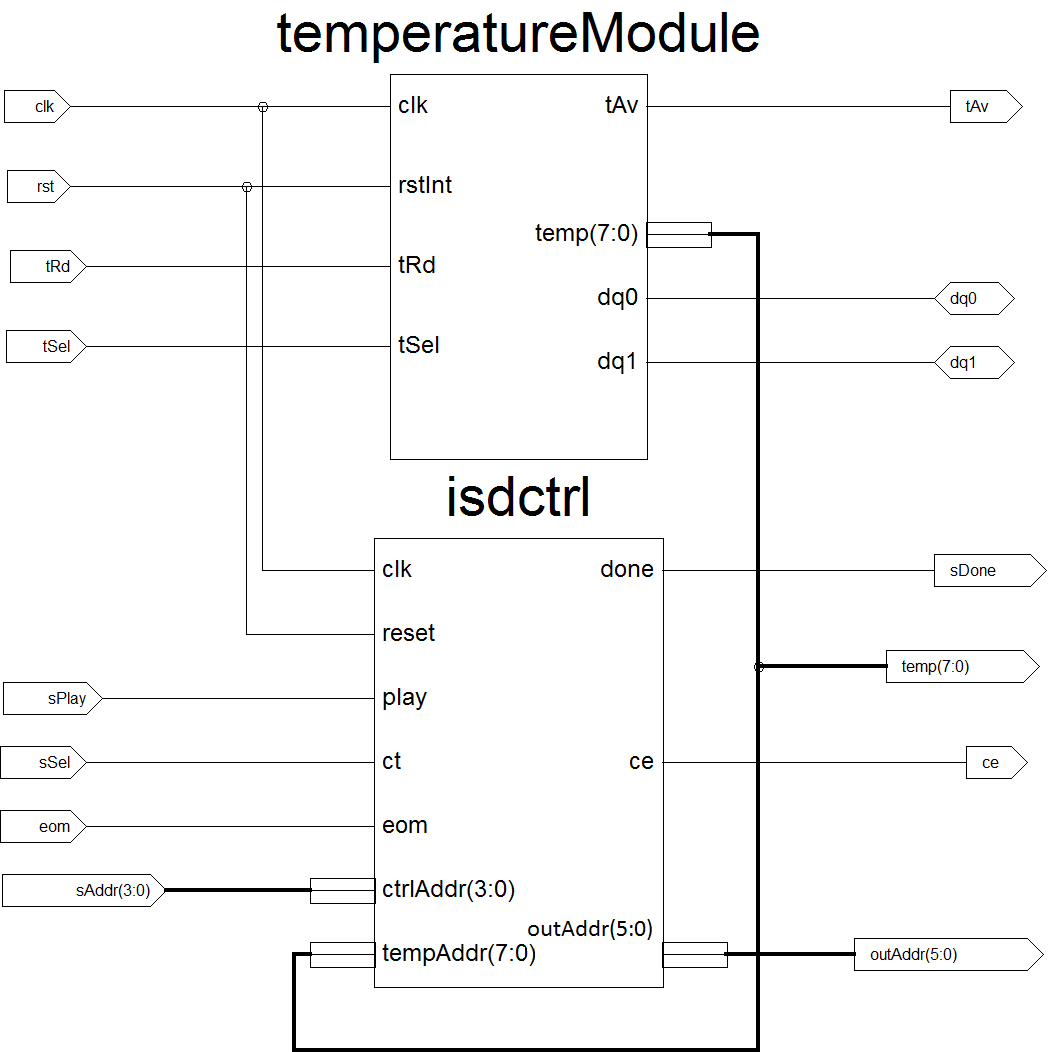
\includegraphics[scale=0.40, angle=0]{Xilinx_CPLD2.png}
			\label{fig:BlockDiagram2}
		  	\caption{Internt blockschema, moduler (CPLD2)}
		\end{figure}	
	
	\section{Komponentlista}
	\label{sec:komponentlistasec}
	\begin{table} [H]
	\caption{Komponentlista, tabell} 
	\label{tab:komponentlista}
	\begin{tabular}{l l l l}
		
		{\bf Komponenter}
		\\{Part} & {Value} & {Device} & {Manufacturer} \\
		\hline
C1-C5, C8 & 100n & capacitor & - \\
C6 & 22u & capacitor & -  \\
C7 & 4u7 & capacitor & -  \\
LED1-LED13 & - & led & -  \\
Q1 & 3.579545MHz & crystal & -  \\
R1-R2, R19, R21 & 4k7 & resistor & -  \\
R3-R14, R22 & 1k5 & resistor & -  \\
R15 & 1k & resistor & -  \\
R16, R23 & 10k & resistor & -  \\
R17 & 470k & resistor & -  \\
R18 & 390k & resistor & -  \\
R20 & 5k1 & resistor & -  \\
R24 & 15k & resistor & -  \\
S1 & - & switch & -  \\
SW1 & - & speaker \\
U1 & - & DS18S20 & Maxim  \\
U2 & - & DS18S20 & Maxim  \\
U3 & - & MT8880C & Mitel  \\
U4 & - & ISD2560 & Futurlec  \\

	\end{tabular}
	\end{table}

	\section{Kretsschema}
		\label{sec:kretsschema}
		\begin{figure}[H]
		  \centering
		      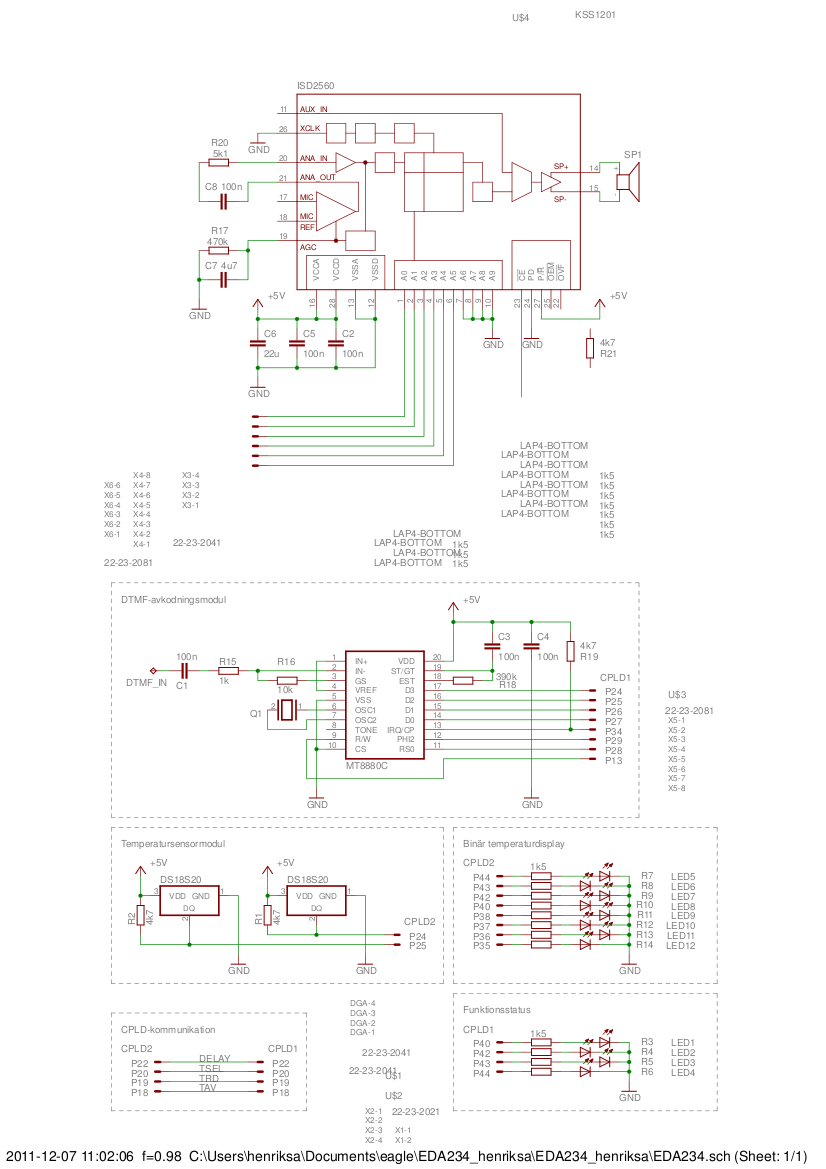
\includegraphics[scale=0.65, angle=90]{schema.png}
		  	\caption{Kretsschema}
		  	\label{fig:schema}
		\end{figure}

	\section{Kretskortslayout}

	\begin{figure}[H]
	  \centering
	      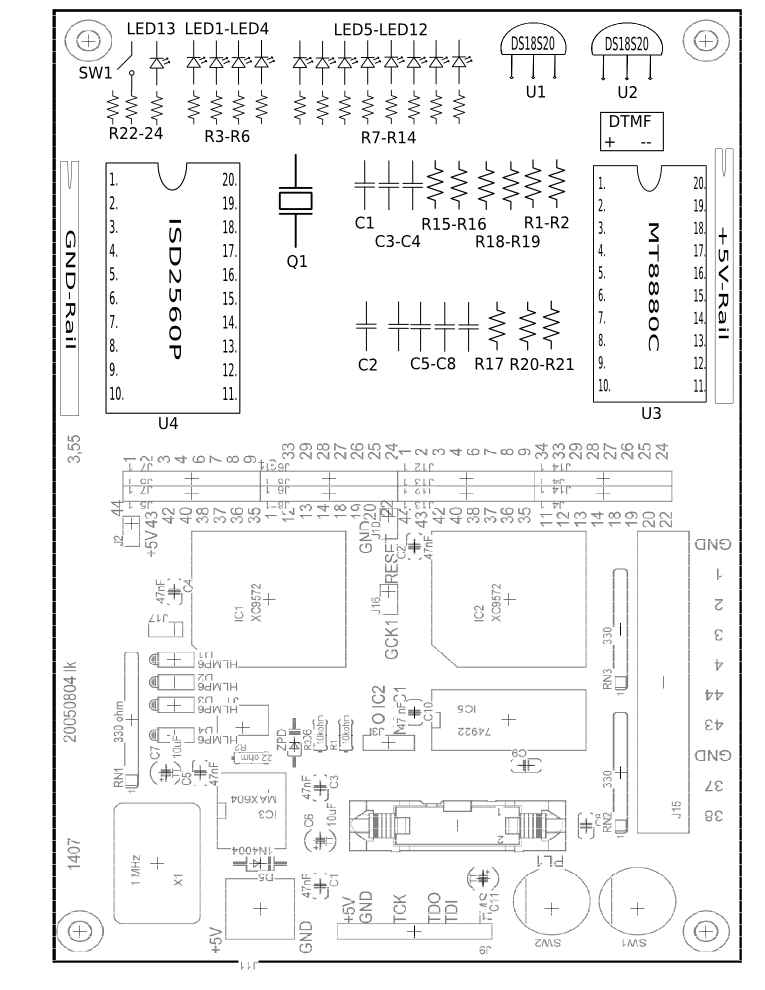
\includegraphics[scale=0.60, angle=0]{Layout.png}
		\label{fig:layout}
	  	\caption{Kretskortslayout}
	\end{figure}
	
	\section{Timingdiagram}

		\begin{figure}[H]
		  \centering
		      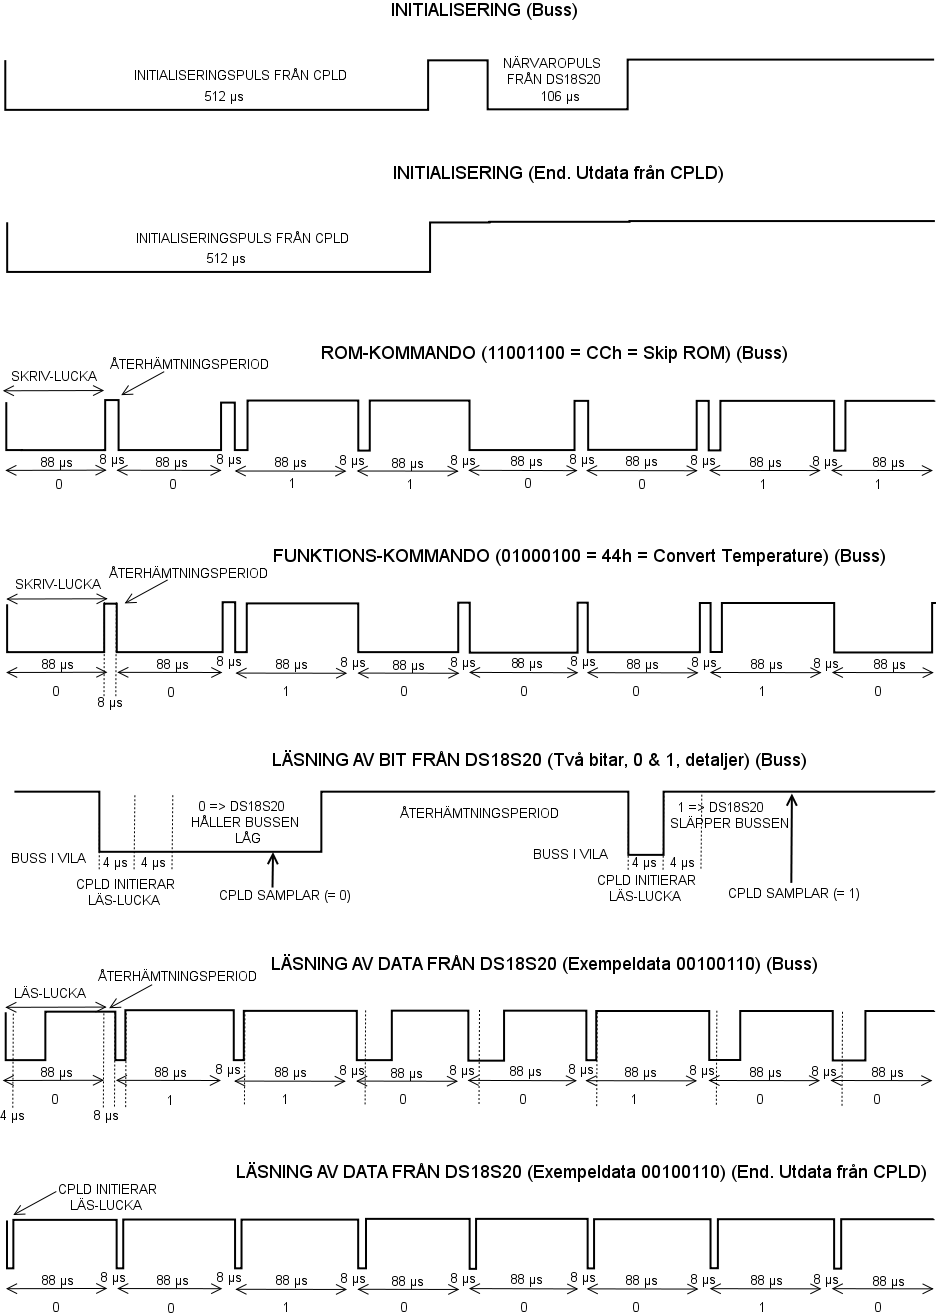
\includegraphics[scale=0.38, angle=0]{TempTiming.png}
			\label{fig:TempTiming}
		  	\caption{Timingdiagram för Temperaturmodulen}
		\end{figure}

	\section{Signallista}
	\begin{table} [H]
	\label{tab:signalTabell}
	\caption{Signallista, tabell} 
	\begin{tabular}{l l l l}
		{\bf Signaler}
		\\{Signal} & {Från} & {Till} & {Beskr.}\\
		\hline
		clk & Extern & Allt & Global Klocksignal\\
		rst & Extern & Allt & Global Resetsignal\\
		buttons[3..0] & Knappsats & Knappsatsmodul & Indatavektor\\
		kbDav & Knappsats & Knappsatsmodul & Availablesignal\\
		funcData[3..0] & Funktionsmodul & FunktionsLEDs & Funktionsstyrning\\
		dtmfData[3..0] & DTMF-Modul & MT8880 & Databuss till MT8880 (bidir.)\\
		\(\Phi\)2 & DTMF-Modul & MT8880 & Klocksignal till MT8880\\
		r/w & DTMF-Modul & MT8880 & Read/Write till MT8880\\
		rs0 & DTMF-Modul & MT8880 & Intieringssignal till MT8880\\
		irq & MT8880 & DTMF-Modul & Interruptsignal från MT8880\\

		kData[3..0] & Knappsatsmodul & Styrenhet & Data från knappsatsmodul\\
		kAv & Knappsatsmodul & Styrenhet & Availablesignal från knappsatsmodul\\
		kAck & Styrenhet & Knappsatsmodul & Ack. till knappsatsmodul\\

		tSel & Styrenhet & Temperaturmodul & Sensorselectsignal\\
		tRd & Styrenhet & Temperaturmodul & Read-signal (starta läsning)\\
		tAv & Temperaturmodul & Styrenhet & Availablesignal, valid data\\

		sData[3..0] & Styrenhet & Ljudmodul & Ljudadressbuss\\
		sSel & Styrenhet & Ljudmodul & Selectsignal för temperatur/ljud\\
		sPlay & Styrenhet & Ljudmodul & Play-signal (spela ljud)\\
		sDone & Ljudmodul & Styrenhet & signalerar uppspelning färdig\\

		dData[3..0] & DTMF-Modul & Styrenhet & DTMF-Databuss\\
		dAv & DTMF-Modul & Styrenhet & Availablesignal från DTMF-Modul\\
		dAck & Styrenhet & DTMF-Modul & Acknowledgement från Styrenhet\\

		fData[3..0] & Styrenhet & Funktionsmodul & Funktionsstatusbuss\\

		dq0 & Temperaturmodul & DS18S20 & Seriell 1-trådsbuss (bidir.)\\
		dq1 & Temperaturmodul & DS18S20 & Seriell 1-trådsbuss (bidir.)\\

		temp[7..0] & Temperaturmodul & Ljudmodul & Temperaturdatabuss\\

		addr[4..0] & Ljudmodul & ISD2560P & Adressbuss till ISD2560P\\
		ce & Ljudmodul & ISD2560P & Chip-Enable från ljudmodul\\
		eom & IDS2560P & Ljudmodul & End-Of-Message från ISD2560P\\\\
	\end{tabular}
	\end{table}
\pagebreak
	\section{Arbetsfördelning}
	\label{sec:arbetsSec}
	
		Det har varit mycket samarbete, där alla samarbetat med alla olika moduler. \\
		Nedan följer en uppdelning i stora drag vem haft det övergripande ansvaret för de större momenten. \\
		Alla har jobbat med felsökning, rapportskrivning och uppkoppling.
	
	\begin{table} [H]
	\caption{Arbetsfördelning, tabell} 
	\label{tab:arbetsTabell}

		\begin{tabular}{l l l l}
		{\bf Arbetsfördelning}
		
		\\{\it Namn} \\ {Moduler / Ansvar} \\ {Övrigt}\\\\
		\hline
				{\it Fredrik Brosser}\\
				 Temperaturmodul, DS18S20, Styrenhet, Funktioner/Knappsats\\
				 Rapport, Blockschema, Tillståndsdiagram\\
				{\it Karl Buchka}\\
				 Ljudmodul, ISD2560P\\
				 Rapport\\
				{\it Andreas Henriksson}\\
				 DTMF-modul, Ljudmodul, Temperaturmodul, MT8880C, ISD2560P\\
				 Rapport, Kretsschema\\
				{\it Johan Wolgers}\\
				 DTMF-modul, MT8880C\\
				 Rapport\\
		\end{tabular}
	\end{table}
\pagebreak
	\section{Datablad}
	
	\label{sec:datablad}
	
	\begin{table} [H]
	\caption{Datablad, tabell} 
	\label{tab:databladsTabell}

		\begin{tabular}{l l}
		{\bf Datablad}
		\\{Krets} & {Datablad}\\
		\hline
			DS18S20 	& {\small \url{http://datasheets.maxim-ic.com/en/ds/DS18S20.pdf}}\\
			ISD2560P 	& {\small \url{http://www.futurlec.com/Others/ISD2560P.shtml}}\\
			MT8880C 	& {\small \url{http://www.cse.chalmers.se/edu/year/2010/course/EDA234/datablad/mt8880.pdf}}\\\\
		\end{tabular}
		\\{\it Länkar uppdaterade 2011-12-11}
	\end{table}

\pagebreak

	\section{Programlistningar}
	\label{sec:programlistningar}	
		\lstinputlisting{TemperatureModule.vhd}
		\lstinputlisting{ControlUnit.vhd}
		\lstinputlisting{DTMFModule.vhd}
		\lstinputlisting{FunctionModule.vhd}
		\lstinputlisting{KeyboardModule.vhd}
		\lstinputlisting{SoundModule.vhd}
\end{document}
